\documentclass[11pt]{beamer}
\usetheme{bars}
\usepackage{xcolor}
\usepackage[utf8x]{inputenc}
\usepackage{ucs}
\usepackage[spanish]{babel}
\usepackage{amsmath}
\usepackage{amsfonts}
\usepackage{multirow}
\usepackage{amssymb}
\usepackage{fancybox}
\usepackage{multicol}
\usepackage{graphicx}
\usepackage{multicol}
\graphicspath{{Figures/}}
%\setbeamercovered{transparent} 
\definecolor{colorZ}{RGB}{0,60,127}
\usecolortheme[RGB={0,60,127}]{structure}
\setbeamertemplate{navigation symbols}{}
\setbeamercolor{mycolor}{bg=colorZ,fg=white}
\defbeamertemplate*{footline}{shadow theme}{%
\leavevmode%
\hbox{\begin{beamercolorbox}[wd=.5\paperwidth,ht=2.5ex,dp=1.125ex,leftskip=.3cm plus1fil,rightskip=.3cm]{author in head/foot}%
    \usebeamerfont{author in head/foot}\hfill\insertshortauthor
\end{beamercolorbox}%
\begin{beamercolorbox}[wd=.43\paperwidth,ht=2.5ex,dp=1.125ex,leftskip=.3cm,rightskip=.3cm plus1fil]{title in head/foot}%
    \usebeamerfont{title in head/foot}\insertshorttitle\hfill%
\end{beamercolorbox}%
\begin{beamercolorbox}[wd=.07\paperwidth,ht=2.5ex,dp=1.125ex,leftskip=.1cm,rightskip=.1cm plus1fil]{mycolor}%
\hfill\insertframenumber\,/\,\inserttotalframenumber
\end{beamercolorbox}}%
\vskip0pt%
}
\author[Daniel Osorio]{\vspace*{-0.55cm}\\\normalsize{\scriptsize{Presented by:}\\\normalsize{\textbf{Daniel Camilo Osorio Hurtado}}}\\\scriptsize{in partial fulfillment of requirements for the degree of} \normalsize{\\\textbf{Master in Bioinformatics}\newline \newline Advisors: \textbf{Janneth Gonzalez PhD.} and \textbf{Andrés Pinzón PhD.}}\\\scriptsize{Bioinformatics and Computational Systems Biology Lab}}
\title[Bioinformatics Master Thesis]{Identifying proteins and metabolic pathways associated to the neuroprotective response mediated by tibolone in astrocytes under an induced inflammatory model}
\date[]{\scriptsize{\vspace{-1.1cm}\\
\includegraphics[scale=.06]{UN}\\\textbf{Universidad Nacional de Colombia\\ Engineering Faculty - Department of Systems and Industrial Engineering\\Bogotá, Colombia}}}
\begin{document}
\maketitle
\section{Introduction}
\begin{frame}{CNS: Central Nervous System}
\begin{center}
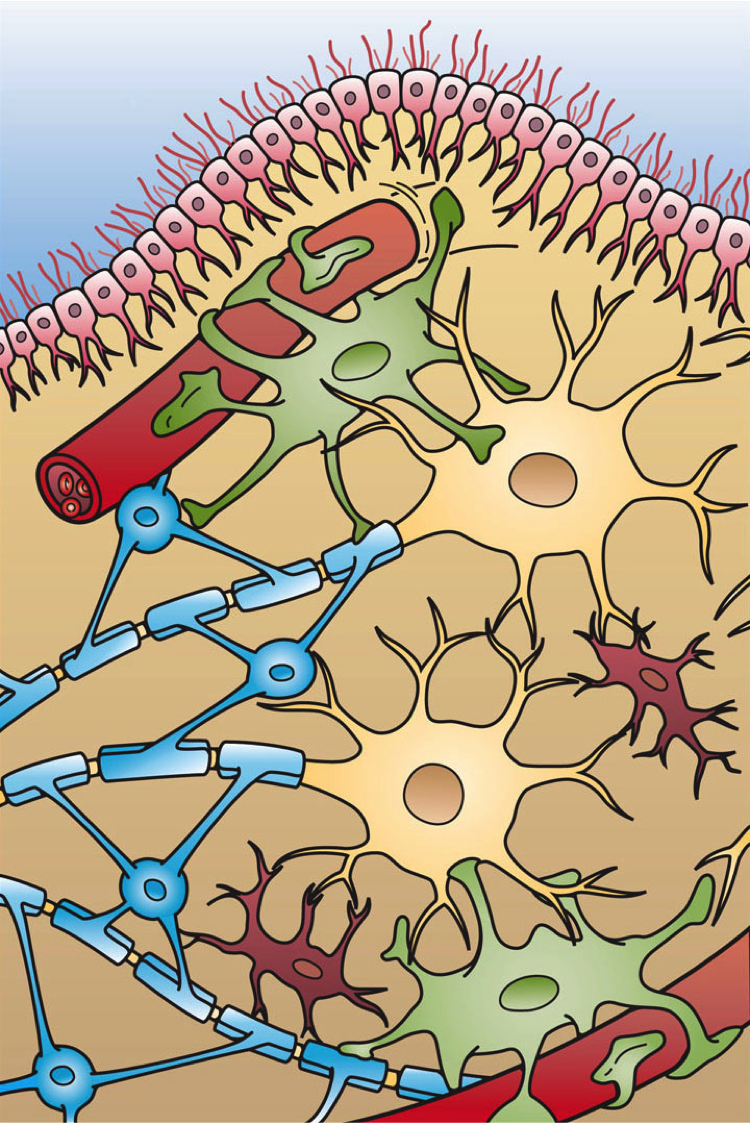
\includegraphics[width=0.4\textwidth]{CNS}\\{\scriptsize \textbf{\textcircled{c} Holly Fischer} artwork.}
\end{center}
\end{frame}
\begin{frame}{Astrocyte - Neuron Metabolic Relationship}
\begin{center}
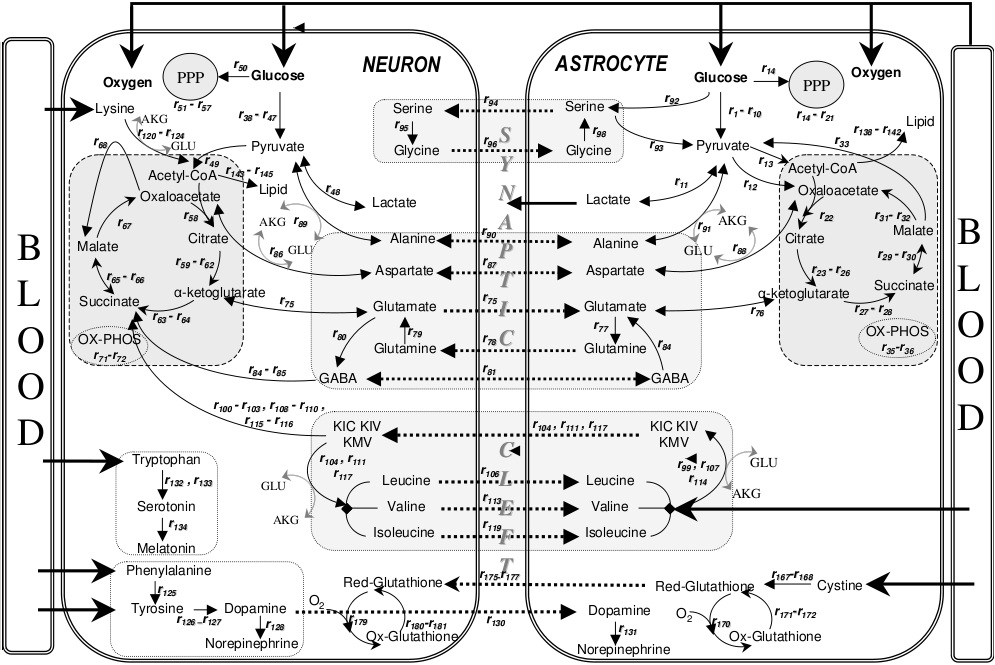
\includegraphics[width=0.82\textwidth]{Relationship}
\end{center}
\begin{scriptsize}
\textbf{Figure from: }Çakir, Tunahan \textit{et al.}, (2007). Reconstruction and flux analysis of coupling between metabolic pathways of astrocytes and neurons: application to cerebral hypoxia.\\
\end{scriptsize}
\end{frame}
\begin{frame}{Astrocytes Metabolic Functions}
\begin{center}
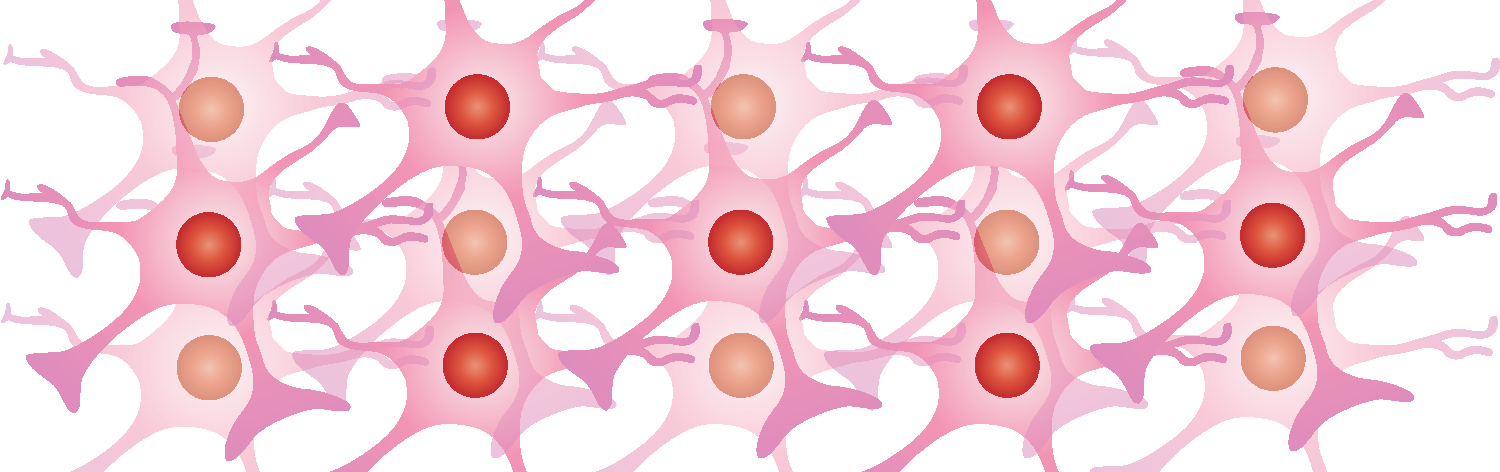
\includegraphics[width=\textwidth]{GFAP}
\end{center}
\begin{center}
\fcolorbox{cyan}{cyan}{\strut \textcolor{white}{\textbf{K$^{+}$} Membrane Potential}} \pause
\fcolorbox{cyan}{cyan}{\strut \textcolor{white}{\textbf{Ca$^{+2}$} signaling}} \pause
\fcolorbox{cyan}{cyan}{\strut \textcolor{white}{\textbf{Lactate} release}} \pause
\fcolorbox{cyan}{cyan}{\strut \textcolor{white}{[\textbf{DOPA}], [\textbf{Glu}], [\textbf{GABA}], [\textbf{Gly}] and [\textbf{Cys}] regulator}} \pause
\fcolorbox{cyan}{cyan}{\strut \textcolor{white}{\textbf{pH} maintenance}} \pause
\fcolorbox{cyan}{cyan}{\strut \textcolor{white}{\textbf{ROS} detox}} \pause
\fcolorbox{cyan}{cyan}{\strut \textcolor{white}{\textbf{Gln}, \textbf{ATP} and \textbf{D-serine} release}}
\end{center}
\end{frame}
\begin{frame}{What is inflammation about?}
\begin{center}
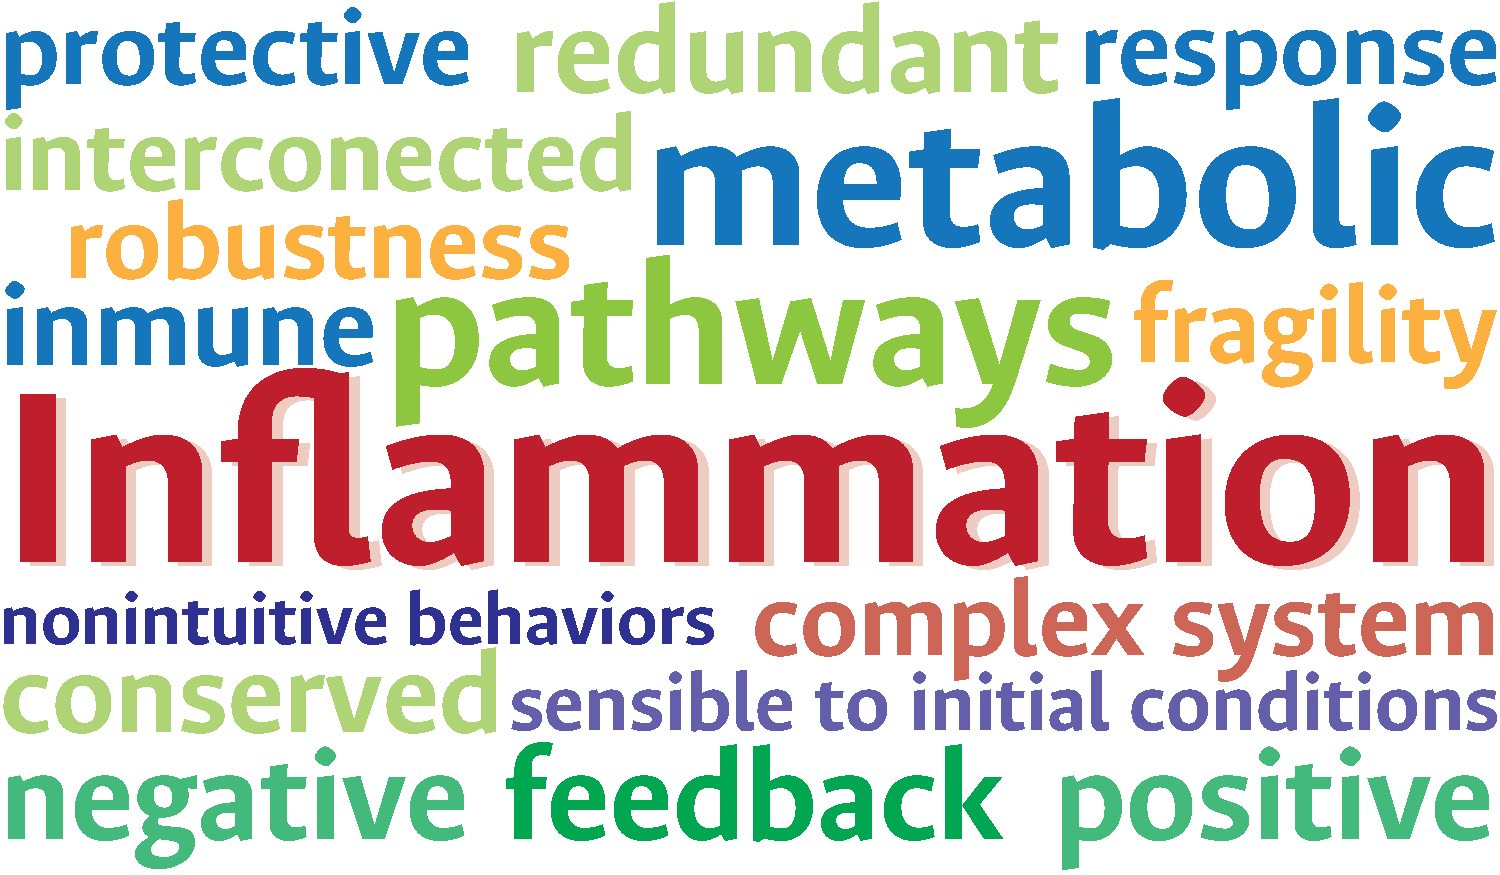
\includegraphics[width=\textwidth]{Inflammation}
\end{center}
\end{frame}
\begin{frame}{CNS inflammation}
\begin{center}
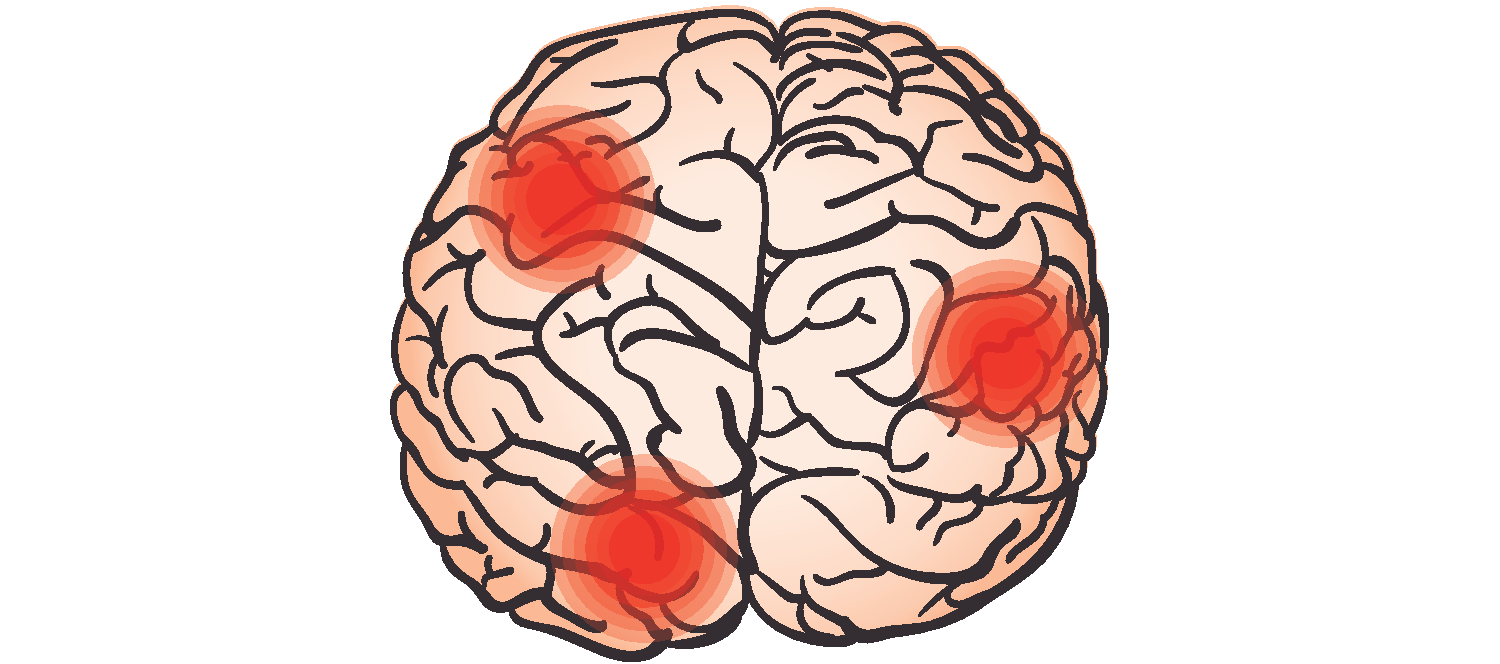
\includegraphics[width=9.5cm]{BInflam}
\end{center}
\begin{center}
\fcolorbox{cyan}{cyan}{\textcolor{white}{\strut Neurodegenerative diseases}}
\fcolorbox{cyan}{cyan}{\textcolor{white}{\strut Cardiovascular events}}
\fcolorbox{cyan}{cyan}{\textcolor{white}{\strut Stress}}
\fcolorbox{cyan}{cyan}{\textcolor{white}{\strut Smoke}}
\fcolorbox{red}{red}{\textcolor{white}{{\strut Obesity (Over Nutrition or Caloric Excess)}}}
\end{center}
\end{frame}
\begin{frame}{Metabolic Inflammation or Metainflammation}
\begin{center}
\fcolorbox{red}{red}{\strut \textcolor{white}{\textbf{Free Fatty Acids (Palmitate)} Increase}}
\end{center}
\begin{center}
\fcolorbox{red}{red}{\strut \textcolor{white}{$\blacktriangle$ IKK$\beta$}} + \fcolorbox{red}{red}{\strut \textcolor{white}{$\blacktriangle$ NF$\kappa\beta$}} $\rightarrow$ \fcolorbox{black}{black}{\strut \textcolor{white}{$\blacktriangledown$ Leptine}} + 
\fcolorbox{black}{black}{\strut \textcolor{white}{$\blacktriangledown$ Insuline}}
\end{center}
\pause
\begin{center}
\fcolorbox{teal}{teal}{\textcolor{white}{\strut $\blacktriangle$ Endoplasmic reticulum stress}} $\rightarrow$ \fcolorbox{red}{red}{\textcolor{white}{\strut $\blacktriangle$ UPR}}
\end{center}
\begin{center}
\fcolorbox{blue}{blue}{\strut \textcolor{white}{$\blacktriangle$ CRP Ligands}}  $\rightarrow$ \fcolorbox{red}{red}{\strut \textcolor{white}{$\blacktriangle$ TNF$\alpha$}} + \fcolorbox{red}{red}{\strut \textcolor{white}{$\blacktriangle$ IL6}} + \fcolorbox{red}{red}{\strut \textcolor{white}{$\blacktriangle$ ROS}} 
\end{center}
\end{frame}
\begin{frame}{Astrogliosis or Reactive Astrocytosis}
\begin{center}
\includegraphics[width=\textwidth]{R}\\
\end{center}
\begin{center}
\fcolorbox{red}{red}{\strut \textcolor{white}{\textbf{ROS} generator}} $\rightarrow$
\fcolorbox{red}{red}{\strut \textcolor{white}{\textbf{Cytokine} production}} \pause\\
\fcolorbox{red}{red}{\strut \textcolor{white}{\textbf{Glu} Excitotoxicity}} $\rightarrow$
\fcolorbox{red}{red}{\strut \textcolor{white}{\textbf{Ca$^{+2}$} uptake}} + 
\fcolorbox{red}{red}{\strut \textcolor{white}{\textbf{Mitochondrial} failure}}
\end{center}
\end{frame}
%\begin{frame}{Translational Bioinformatics: Systems Biology}
%\begin{center}
%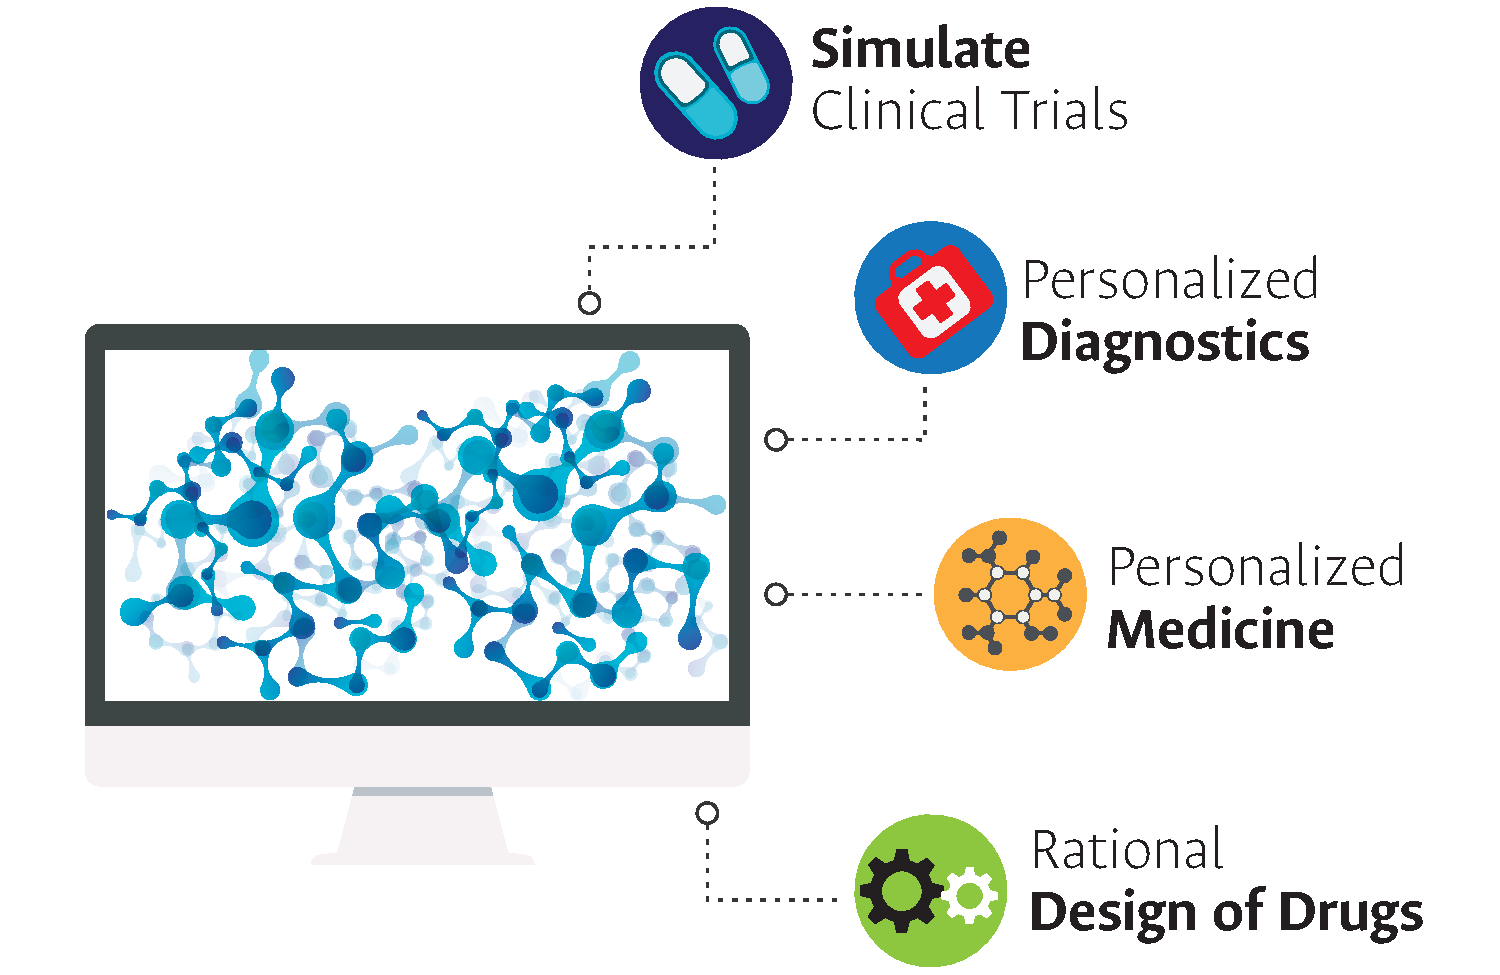
\includegraphics[width=\textwidth]{TMedicine}
%\end{center}
%\end{frame}
\begin{frame}{Inflammation Treatment: Steroids}
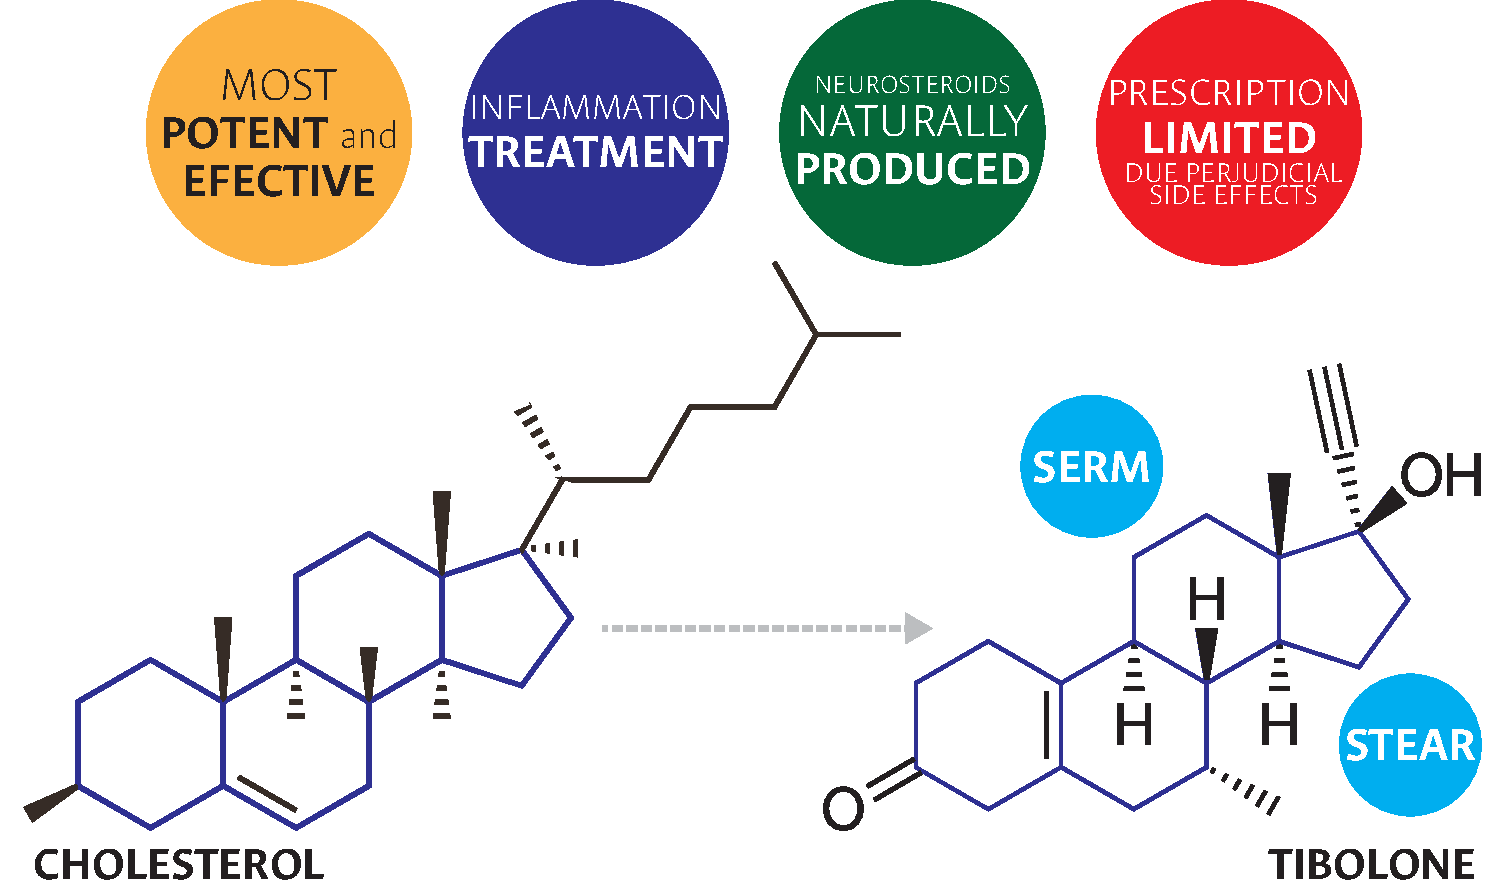
\includegraphics[width=\textwidth]{Steroids}
\begin{center}
{\scriptsize Katarzyna Wojtal, Micha l K. Trojnar, and Stanis law J. Czuczwar. (2006). \textbf{Endogenous neuroprotective factors: neurosteroids.}\\}
\end{center}
\end{frame}
\begin{frame}{Tibolone Metabolism}
\begin{center}
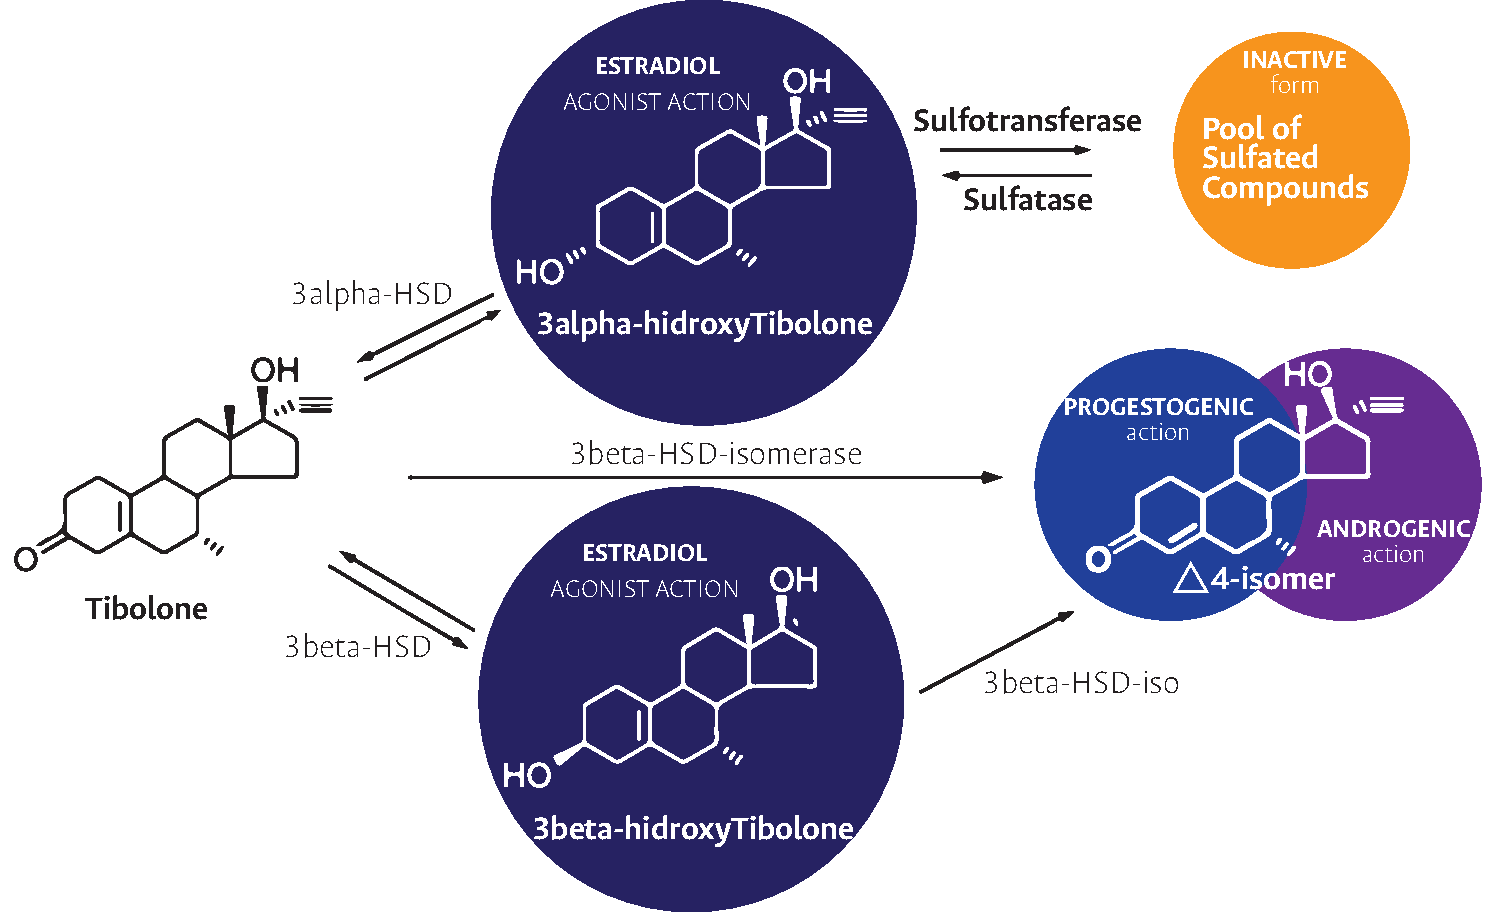
\includegraphics[width=0.95\textwidth]{TiboloneM}
\end{center}
{\scriptsize \textbf{Modified of:} Kloosterboer, H. J. (2004). Tissue-selectivity: the mechanism of action of tibolone.\\}
\end{frame}
\begin{frame}{What effects does tibolone have on Astrocytic inflammatory scenarios?}
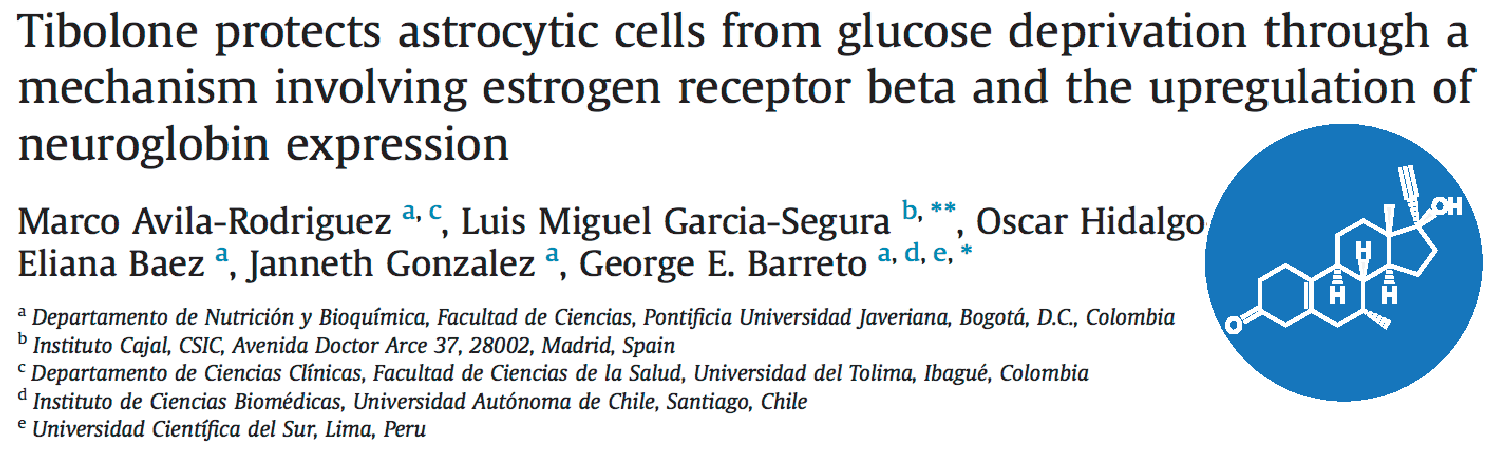
\includegraphics[width=\textwidth]{Tibolone}
\end{frame}
\section{Objectives and Methods}
\begin{frame}{Objectives:}
To identify proteins and metabolic pathways involved in the neuroprotective effects of tibolone in human astrocytes based in metabolic scenarios comparation we set:
\begin{itemize}
\item Build a tissue specific computational model of astrocytes metabolism using gene expression data integration.
\item Evaluate the effects caused by the increase of free fatty acids and tibolone presence in astrocytes metabolism.
\item Determine metabolic pathways and relevant functional products in response to steroid tibolone through systems biology approximations.
\item Evaluate the importance of proteins and metabolic pathways previously identified on the dynamics of the metabolic model.
\end{itemize}
\end{frame}
\begin{frame}
\begin{block}{\textbf{OBJECTIVE 1:}}
\begin{center}
Build a tissue specific computational model of \\astrocytes metabolism using gene expression data integration.
\end{center}\end{block}
\end{frame}
\begin{frame}{Metabolism Simulation: Flux Balance Analysis (FBA)}
\begin{center}
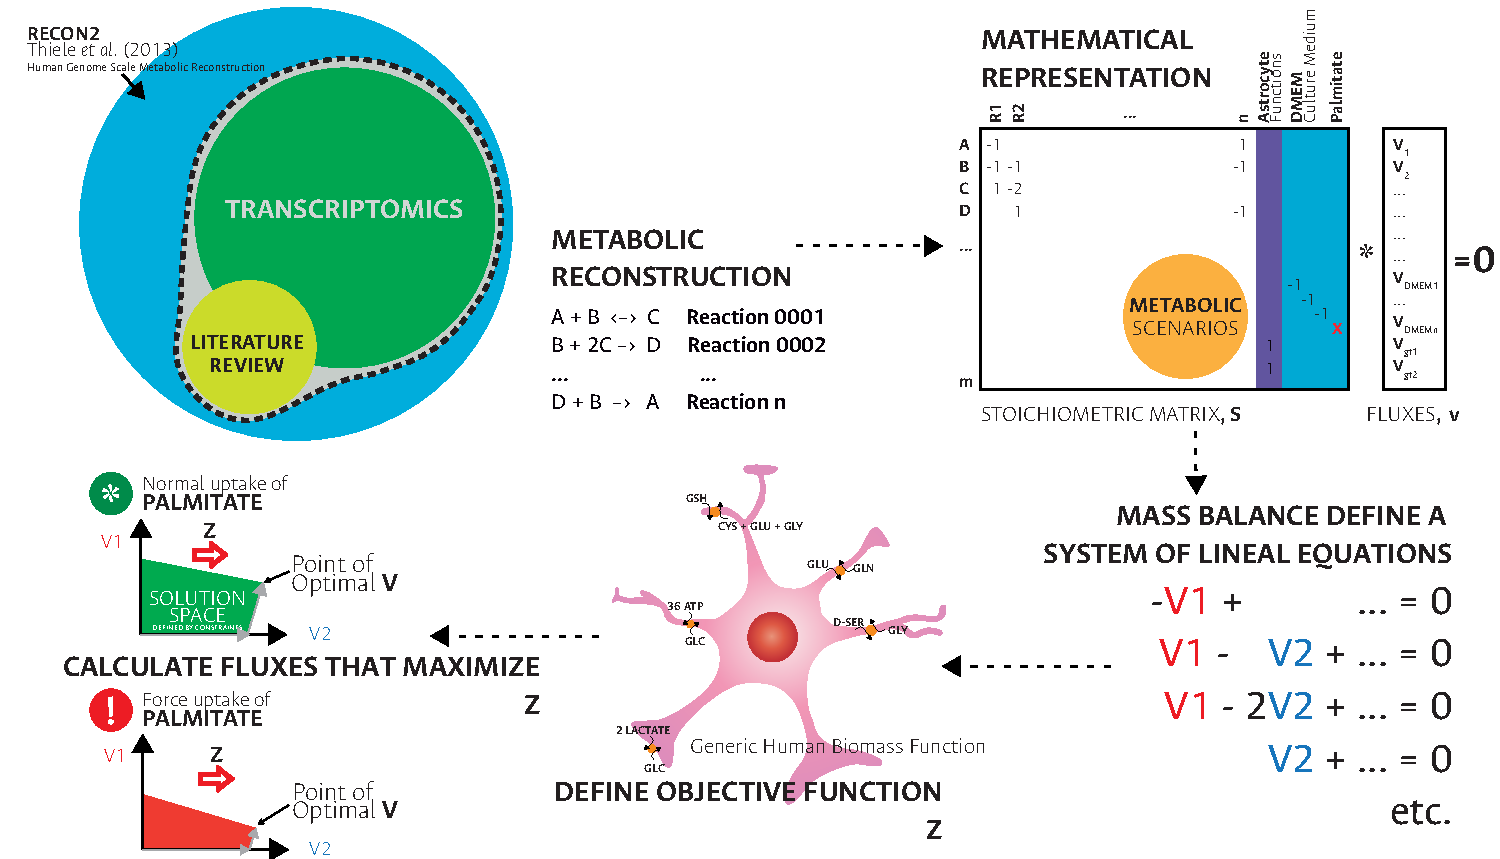
\includegraphics[width=\textwidth]{FBA}
\end{center}
{\scriptsize \textbf{Modified  of:} Orth, J. D., Thiele, I., and  Palsson, B. Ø. (2010). What is flux balance analysis?.\\}
\end{frame}
\begin{frame}{Healthy Human Astrocytes Gene Expression Data}
\begin{center}
\begin{multicols}{2}
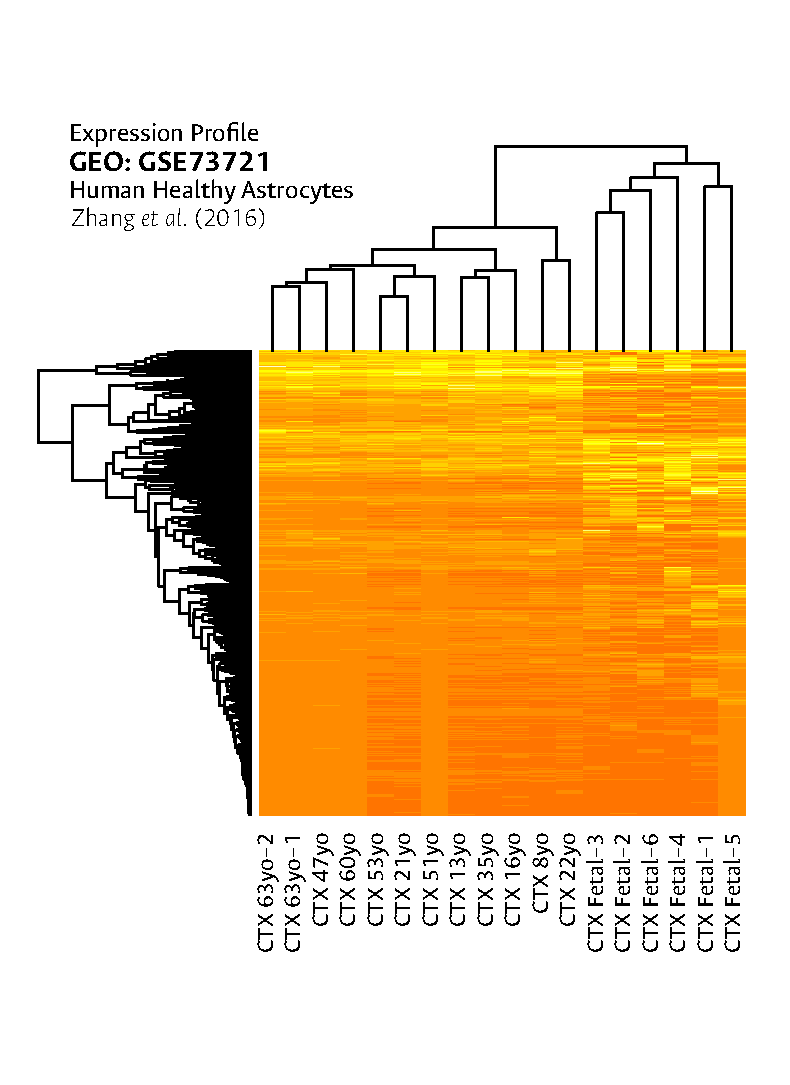
\includegraphics[width=5cm]{GE}\\
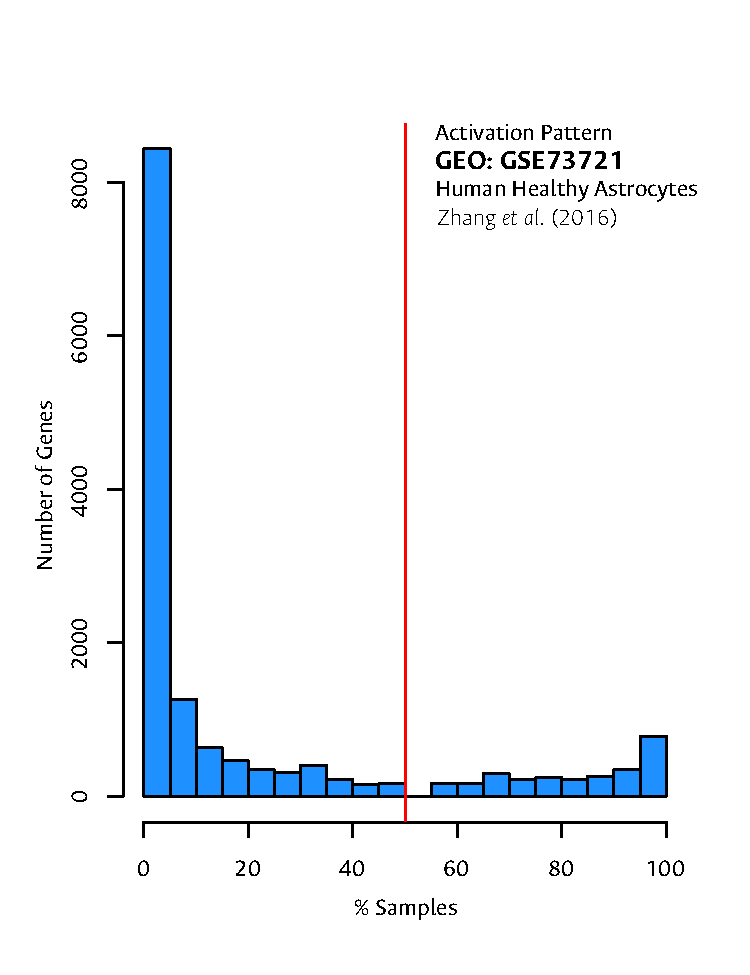
\includegraphics[width=5cm]{ActiveGenes}
\end{multicols}
\end{center}
\end{frame}
\begin{frame}{Mapping Reactions}
\begin{center}
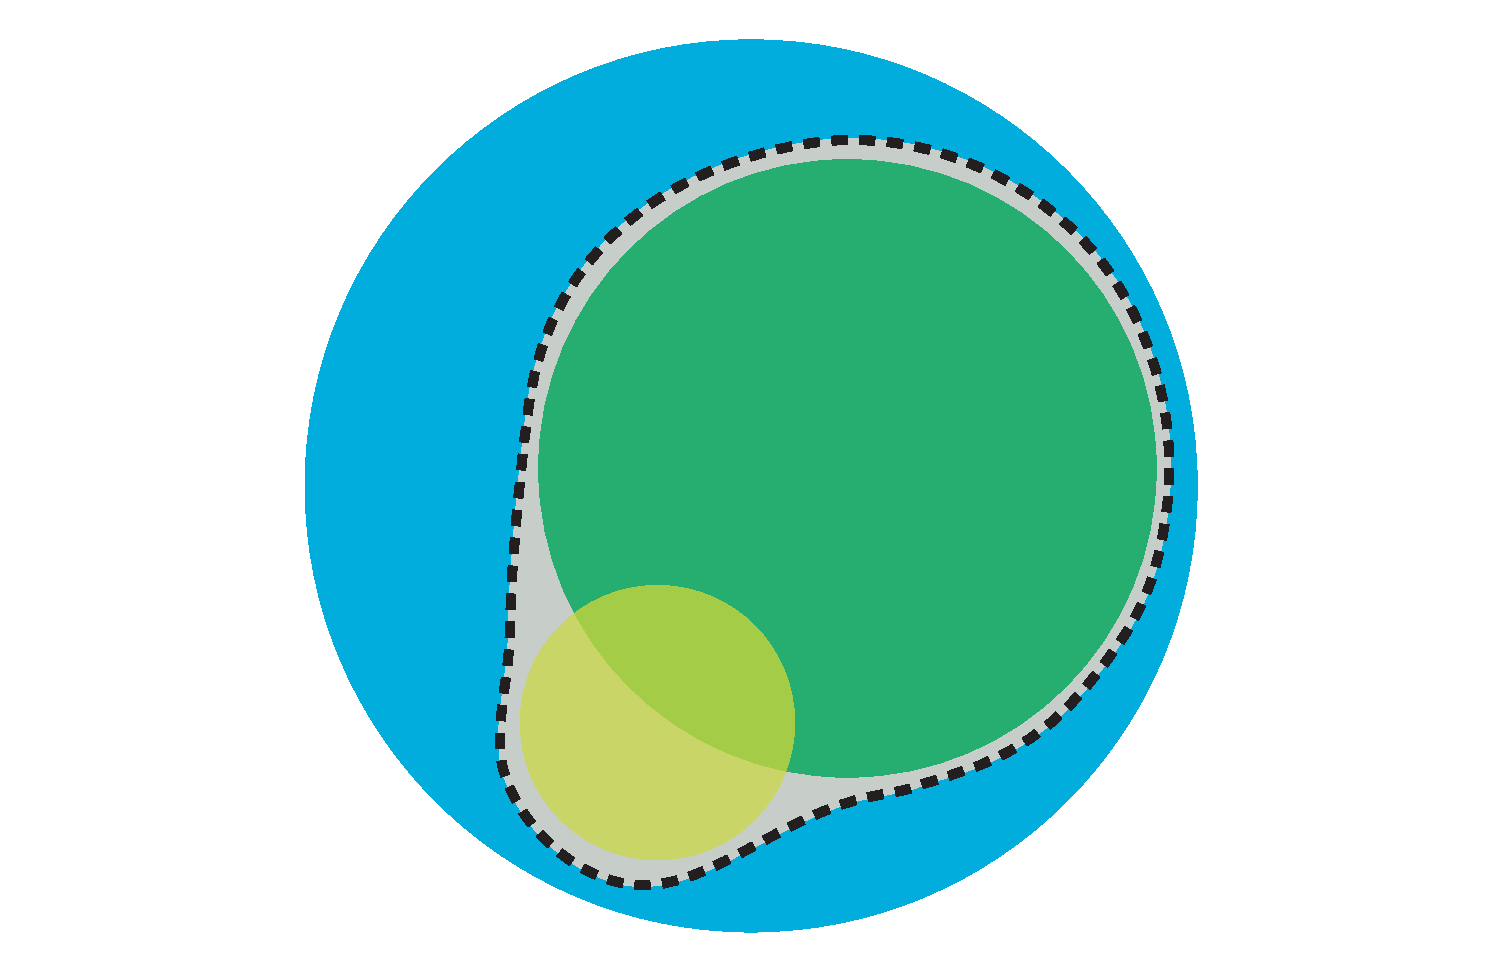
\includegraphics[width=\textwidth]{TSR}
\end{center}
\end{frame}
\begin{frame}{Gap-Find and Gap-Fill Available Algorithms}
\begin{center}
\begin{tabular}{r|c|p{3.7cm}}
\hline
\textbf{ALGORITHM}&\textbf{ENVIRONMENT}&\textbf{HOW IT WORKS}\\
\hline
\hline
\multirow{2}{*}{SMILEY}&\multirow{2}{*}{Python - OpenSource}&· Optimization based.\\
&&· \textbf{Fills one metabolite \emph{per time}}.\\
\hline
\multirow{2}{*}{gap-Find/Fill}&\multirow{2}{*}{GAMS - OpenSource}&· Optimization based.\\
&&· \textbf{Makes several \emph{intra model modifications}}.\\
\hline
\multirow{2}{*}{growMatch}&\multirow{2}{*}{Python - OpenSource}&· Optimization based.\\
&&· \textbf{Fills one objective function \emph{per time}}.\\
\hline
\multirow{2}{*}{fastGapFill}&\multirow{2}{*}{MATLAB - \textbf{Privative}}&· Optimization based.\\
&&· Multiobjective.\\
\hline
\end{tabular}
\end{center}
\end{frame}
\begin{frame}{Finding and Filling Gaps}
\begin{center}
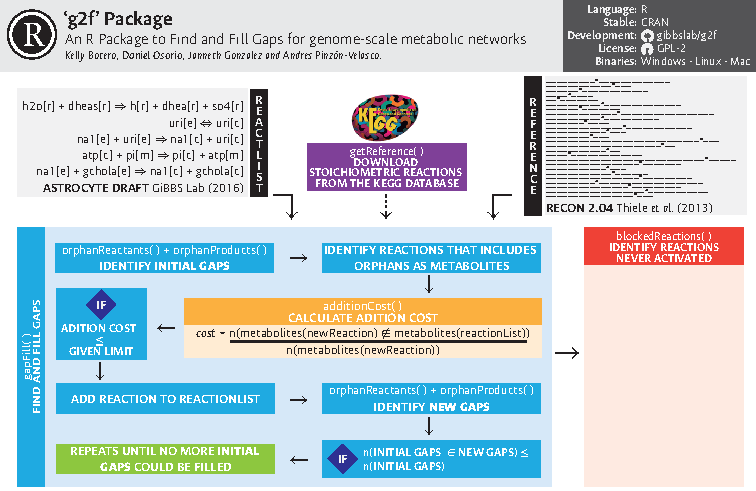
\includegraphics[width=\textwidth]{g2f}
\end{center}
\end{frame}
\begin{frame}{Syntax, Mass-Charge Validation and SBML files}
\begin{center}
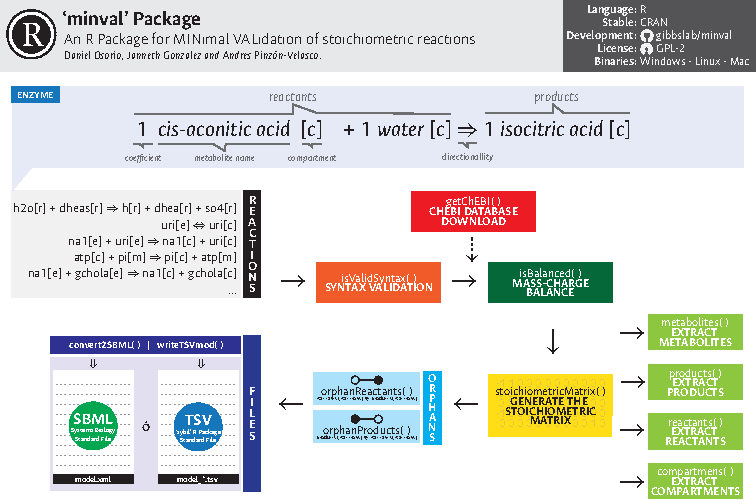
\includegraphics[width=\textwidth]{minval}
\end{center}
\end{frame}
\begin{frame}{Metabolic Model Debugging}
\begin{center}
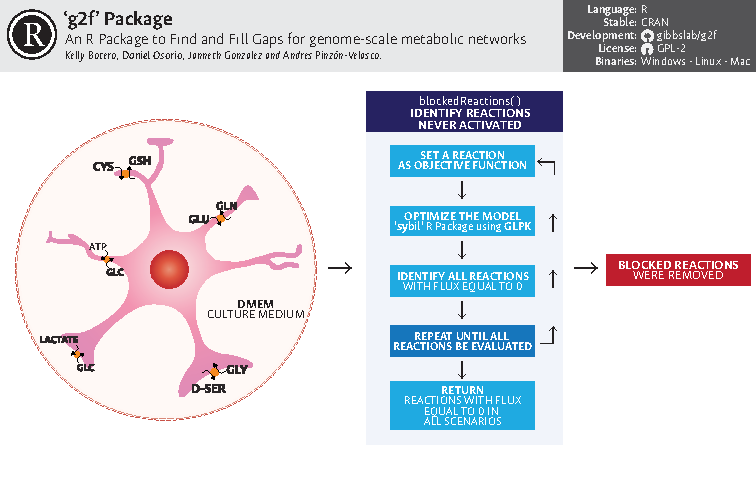
\includegraphics[width=\textwidth]{Debug}
\end{center}
\end{frame}
\begin{frame}{Gene Expression Integration Available Methods}
\begin{center}
\begin{tabular}{r|p{3cm}|p{4.7cm}}
\hline
\textbf{METHOD}&\textbf{ENVIRONMENT}&\textbf{HOW IT WORKS}\\
\hline
\hline
\multirow{2}{*}{GIMME}&\multirow{2}{*}{\parbox{3cm}{\centering{MATLAB  \textbf{Privative}}}}&·{\footnotesize \textbf{Binary Disctretization}}\\
&&·{\footnotesize  \textbf{Ensures flux for a selected objective function}}\\
\hline
\multirow{2}{*}{iMAT}&\multirow{2}{*}{\parbox{3cm}{\centering{MATLAB  \textbf{Privative}}}}&· {\footnotesize Integration proportional to gene-expression (H, M and L categorization)} \\
&&· {\footnotesize Not objective function required} \\
\hline
\multirow{2}{*}{E-FLUX}&\multirow{2}{*}{\textbf{Not implemented}}&· {\footnotesize \textbf{Requires a user-given threshold}}\\
&&· {\footnotesize  Continuous Integration}\\
\hline
\multirow{2}{*}{PROM}&\multirow{2}{*}{\parbox{3cm}{\centering{MATLAB  \textbf{Privative}}}}&·{\footnotesize \textbf{Requires a user-given regulatory network}}\\
&&· {\footnotesize Constraints are setting according to the associated transcript. factor}\\
\hline
\end{tabular}
\end{center}
\end{frame}
\begin{frame}{Constraining the Metabolic Model}
\begin{center}
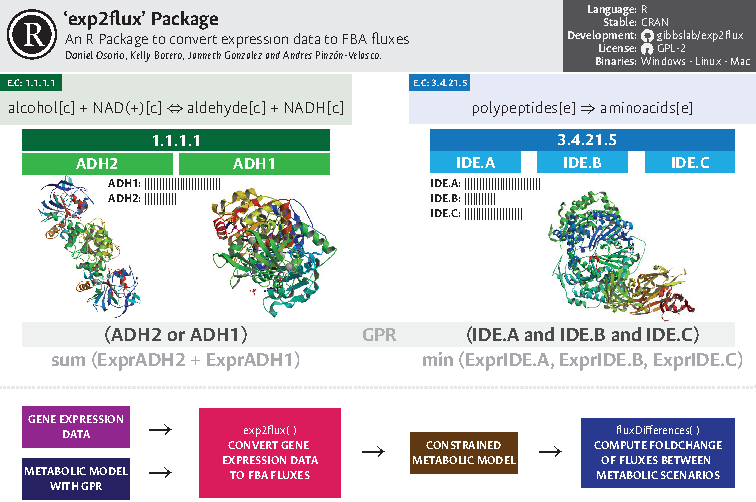
\includegraphics[width=\textwidth]{exp2flux}
\end{center}
\end{frame}
\begin{frame}
\begin{block}{\textbf{OBJECTIVE 2:}}
\begin{center}
Evaluate the effects caused by the increase of free fatty acids and tibolone presence in astrocytes metabolism.\end{center}\end{block}
\end{frame}
\begin{frame}{Metabolic Scenarios}
\begin{center}
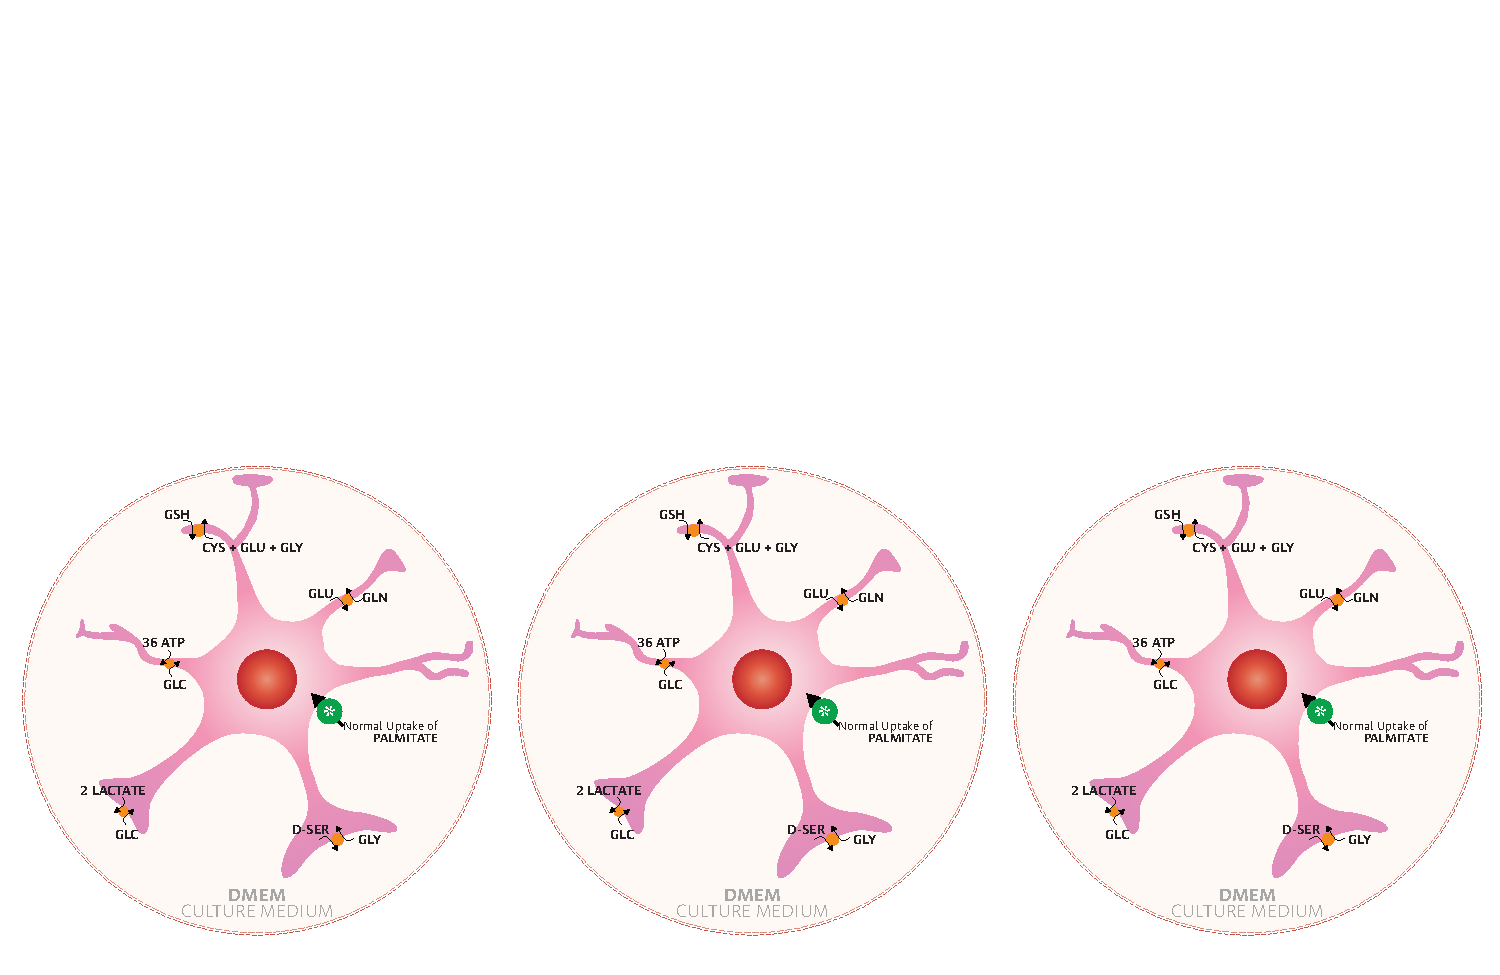
\includegraphics[width=\textwidth]{Healthy}\\
\textbf{MAIN OBJECTIVE FUNCTION:}\\Generic Human Biomass Reaction included in RECON 2.04 \\(Thiele \textit{et al.}, 2013)
\end{center}
\end{frame}
\begin{frame}{Inflamed Metabolic Scenario}
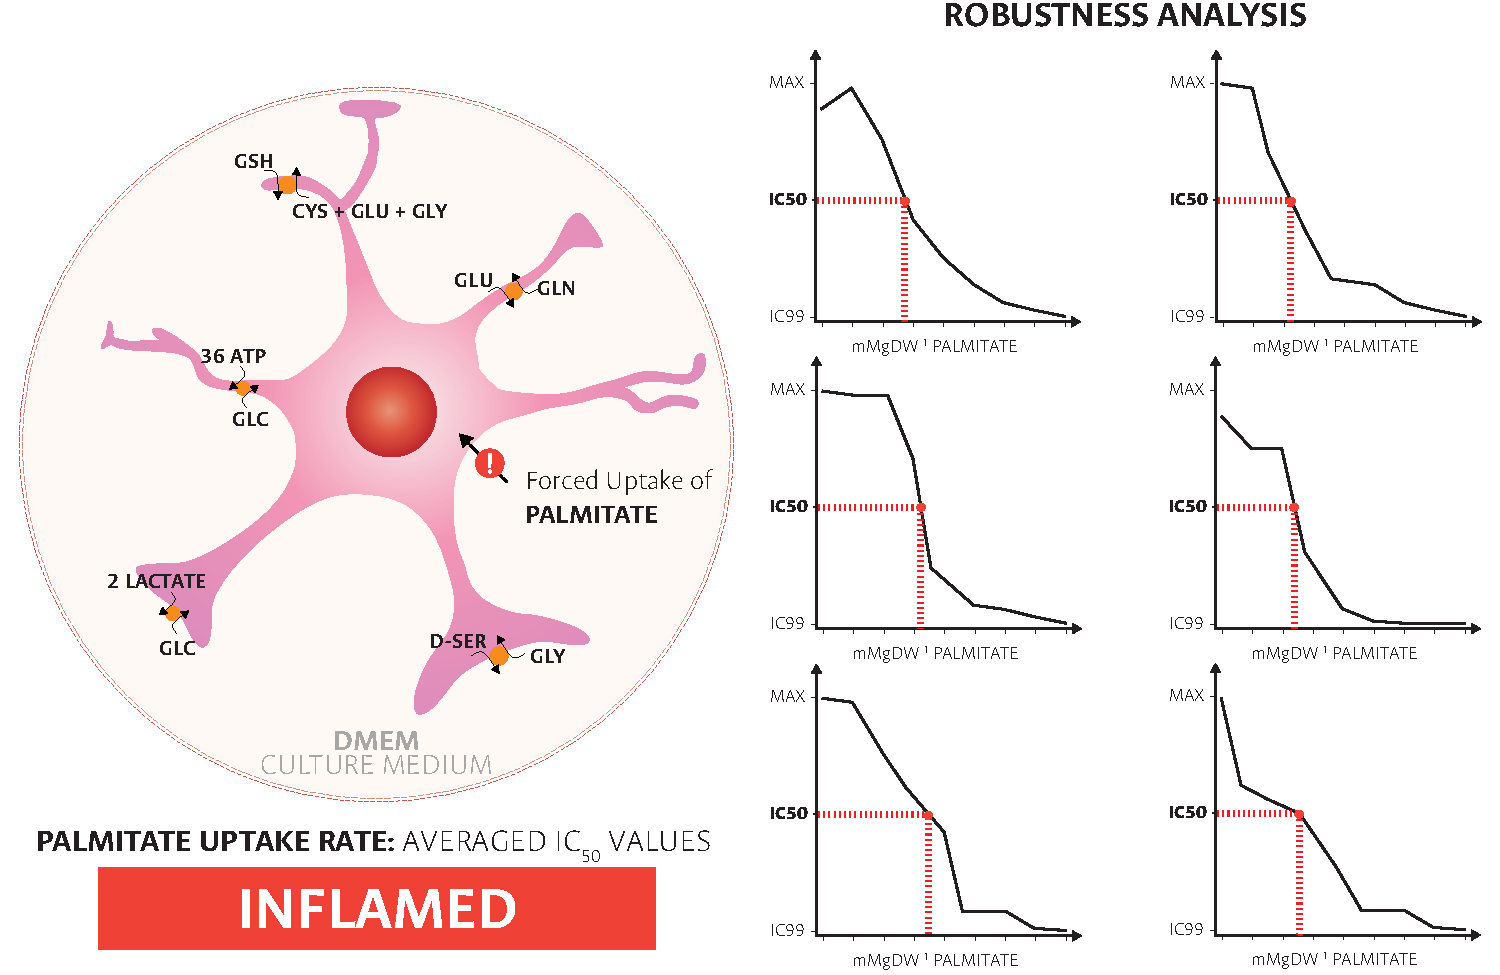
\includegraphics[width=\textwidth]{Inflamed}
\end{frame}
\begin{frame}{Medicated Metabolic Scenario}
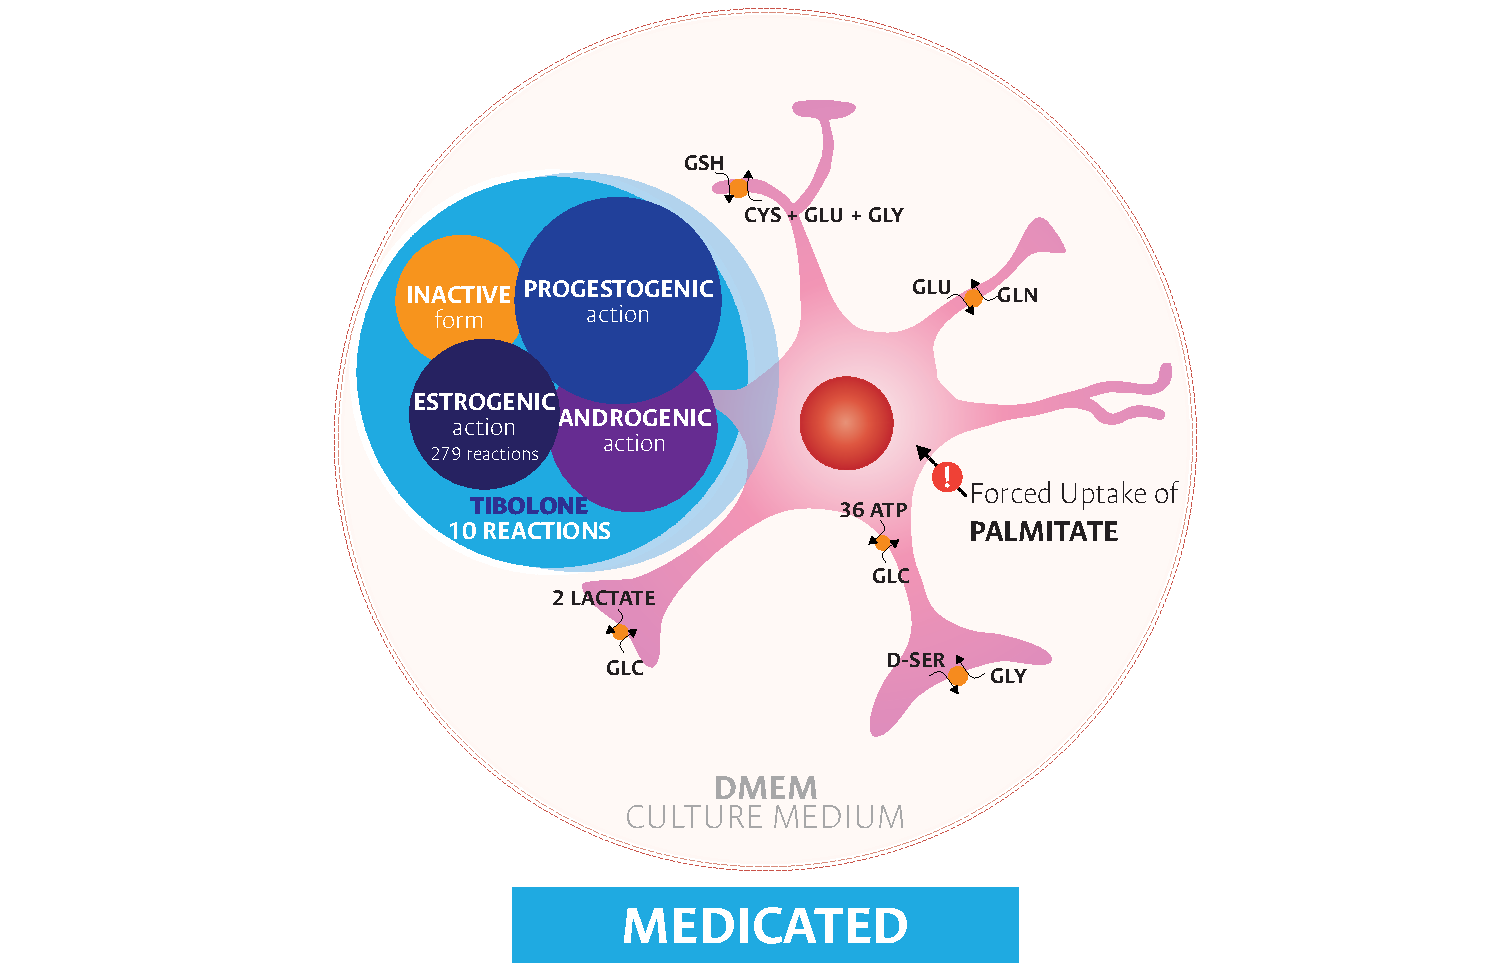
\includegraphics[width=\textwidth]{Medicated}
\end{frame}
\begin{frame}
\begin{block}{\textbf{OBJECTIVE 3:}}
\begin{center}
Determine metabolic pathways and relevant functional products in response to steroid tibolone through systems biology approximations.\end{center}\end{block}
\end{frame}
\begin{frame}{Metabolic Changes}
\begin{center}
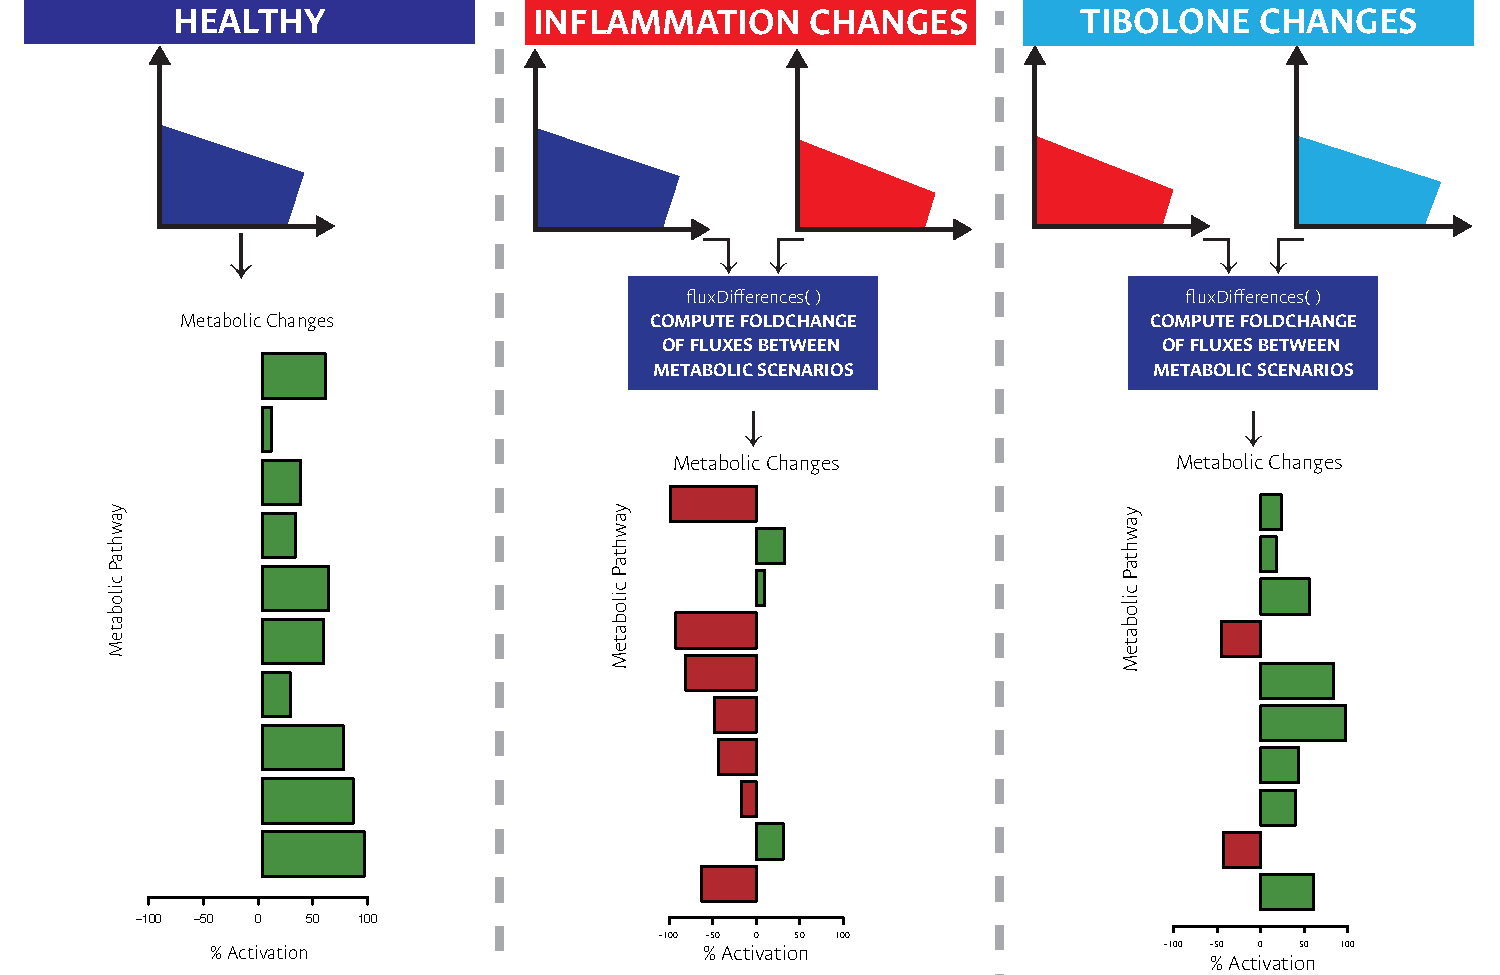
\includegraphics[width=\textwidth]{FluxDifferenes}
\end{center}
\end{frame}
\begin{frame}
\begin{block}{\textbf{OBJECTIVE 4:}}
\begin{center}
Evaluate the importance of proteins and metabolic pathways previously identified on the dynamics of the metabolic model.\end{center}\end{block}
\end{frame}
\begin{frame}{Reaction Knock-out: Protein Importance}
\begin{center}
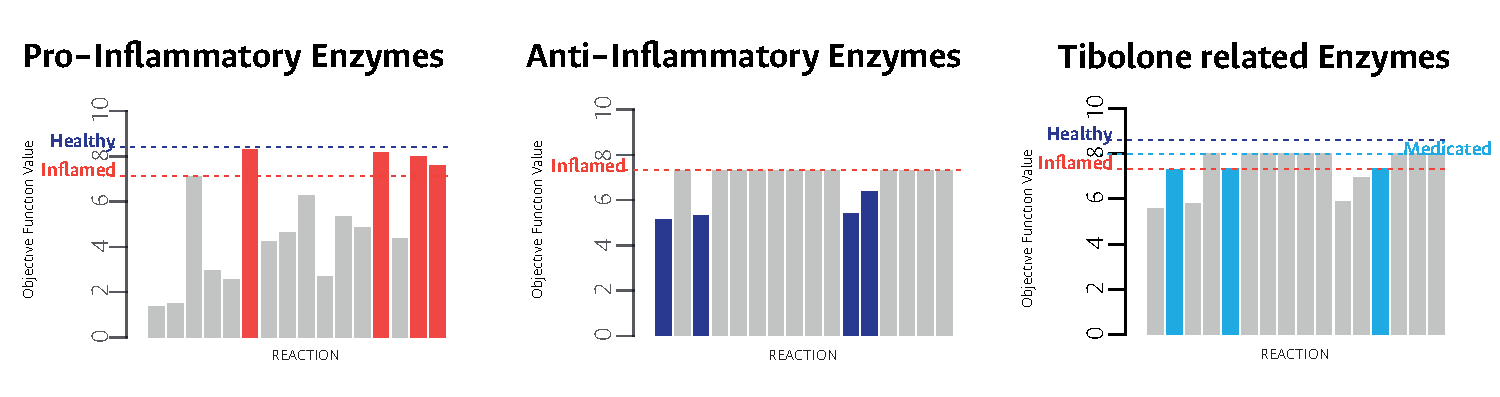
\includegraphics[width=\textwidth]{Networks}
\end{center}
\end{frame}
\section{Results}
\begin{frame}{Tissue Specific Metabolic Reconstruction}
\begin{center}
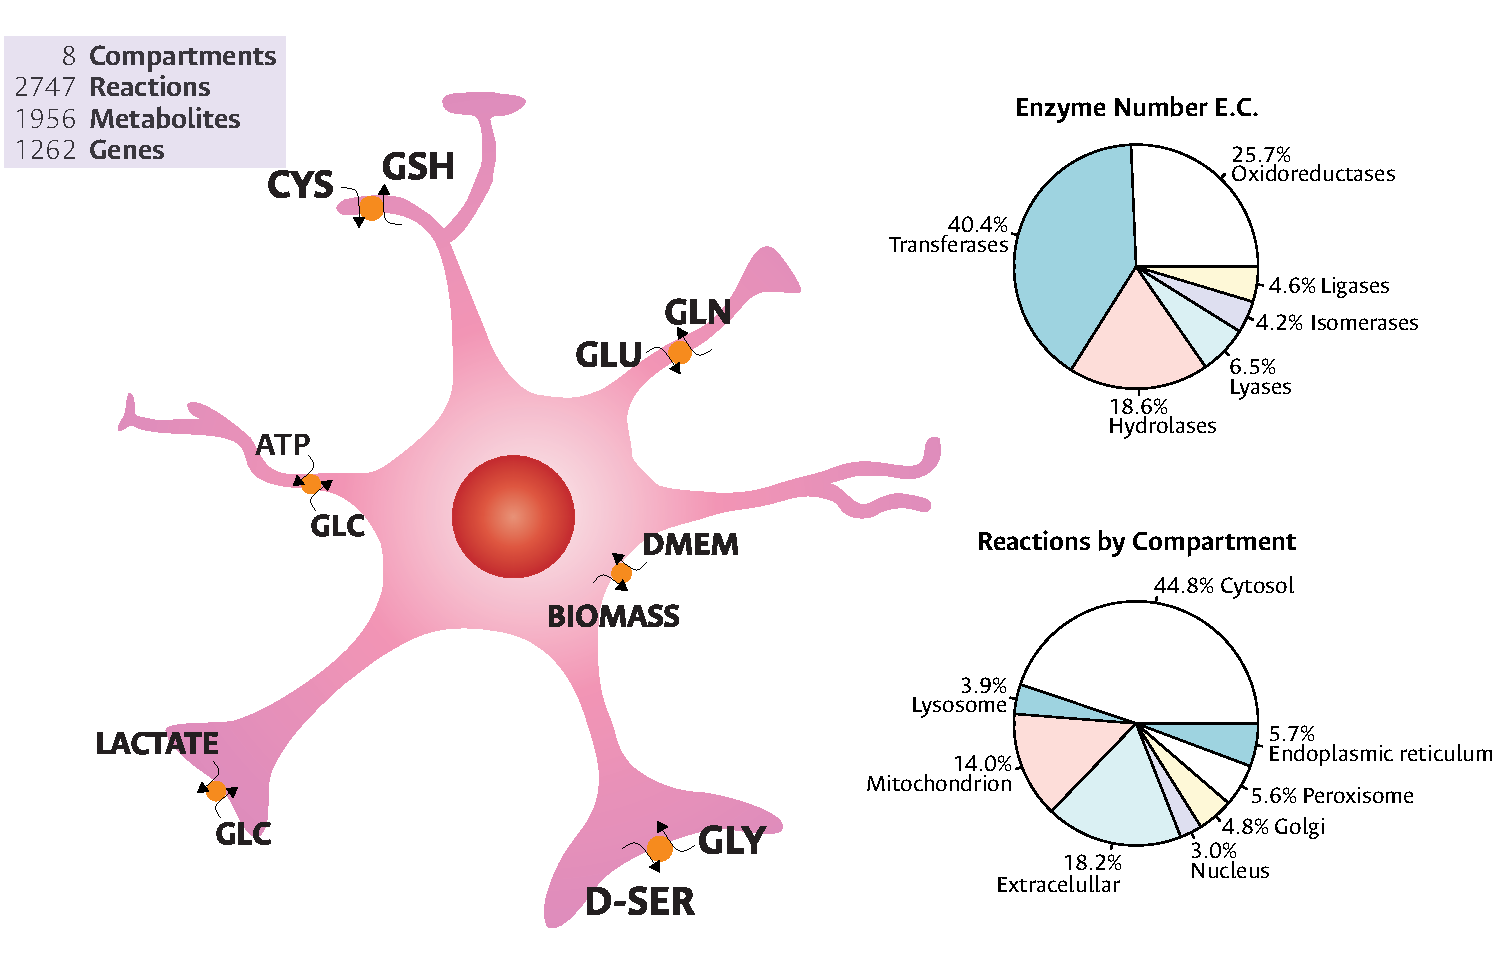
\includegraphics[width=\textwidth]{Astrocyte}
\end{center}
\end{frame}
\begin{frame}{Human Healthy Mature Astrocyte Model}
\begin{center}
\includegraphics[width=\textwidth]{Ages}
\end{center}
\end{frame}
\begin{frame}{Cellular Maintenance: Healthy Scenario}
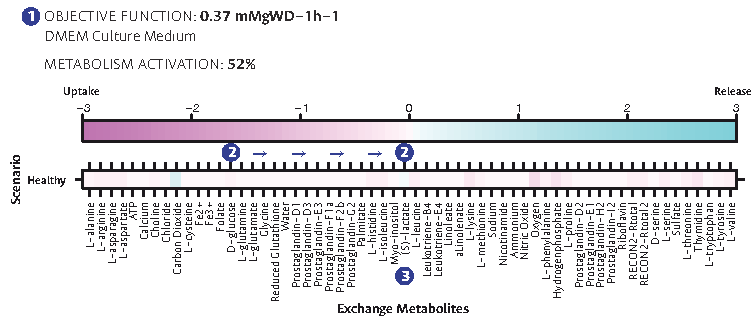
\includegraphics[width=\textwidth]{H-results}\\
\textcolor{blue}{\textcircled{{\tiny 1}}} {\tiny Arabinda Das, \textit{et al}. (2010). Flavonoids activated caspases for apoptosis in human glioblastoma T98G and U87MG cells but not in human normal astrocytes.\vspace{0.2cm}\\}\pause
\textcolor{blue}{\textcircled{{\tiny 2}}}  {\tiny Tunahan Cakir \textit{et al}. (2007). Reconstruction and flux analysis of coupling between metabolic pathways of astrocytes and neurons: application to cerebral hypoxia.\vspace{0.1cm}\\}
\textcolor{blue}{\textcircled{{\tiny 2}}}  {\tiny Rupa Bhowmick, \textit{et al}. (2015). Exploring the diferences in metabolic behavior of astrocyte and glioblastoma: a flux balance analysis approach.\vspace{0.2cm}\\}
\pause
\textcolor{blue}{\textcircled{{\tiny 3}}}  {\tiny Christelle Le Foll, et al. (2010). Fatty acid-induced astrocyte ketone production and the control of food intake.\\}
\end{frame}
\begin{frame}{Averaged IC50:  0.208 $\pm$ 0.024 mMgDW$^{-1}$h$^{-1}$}
\begin{center}
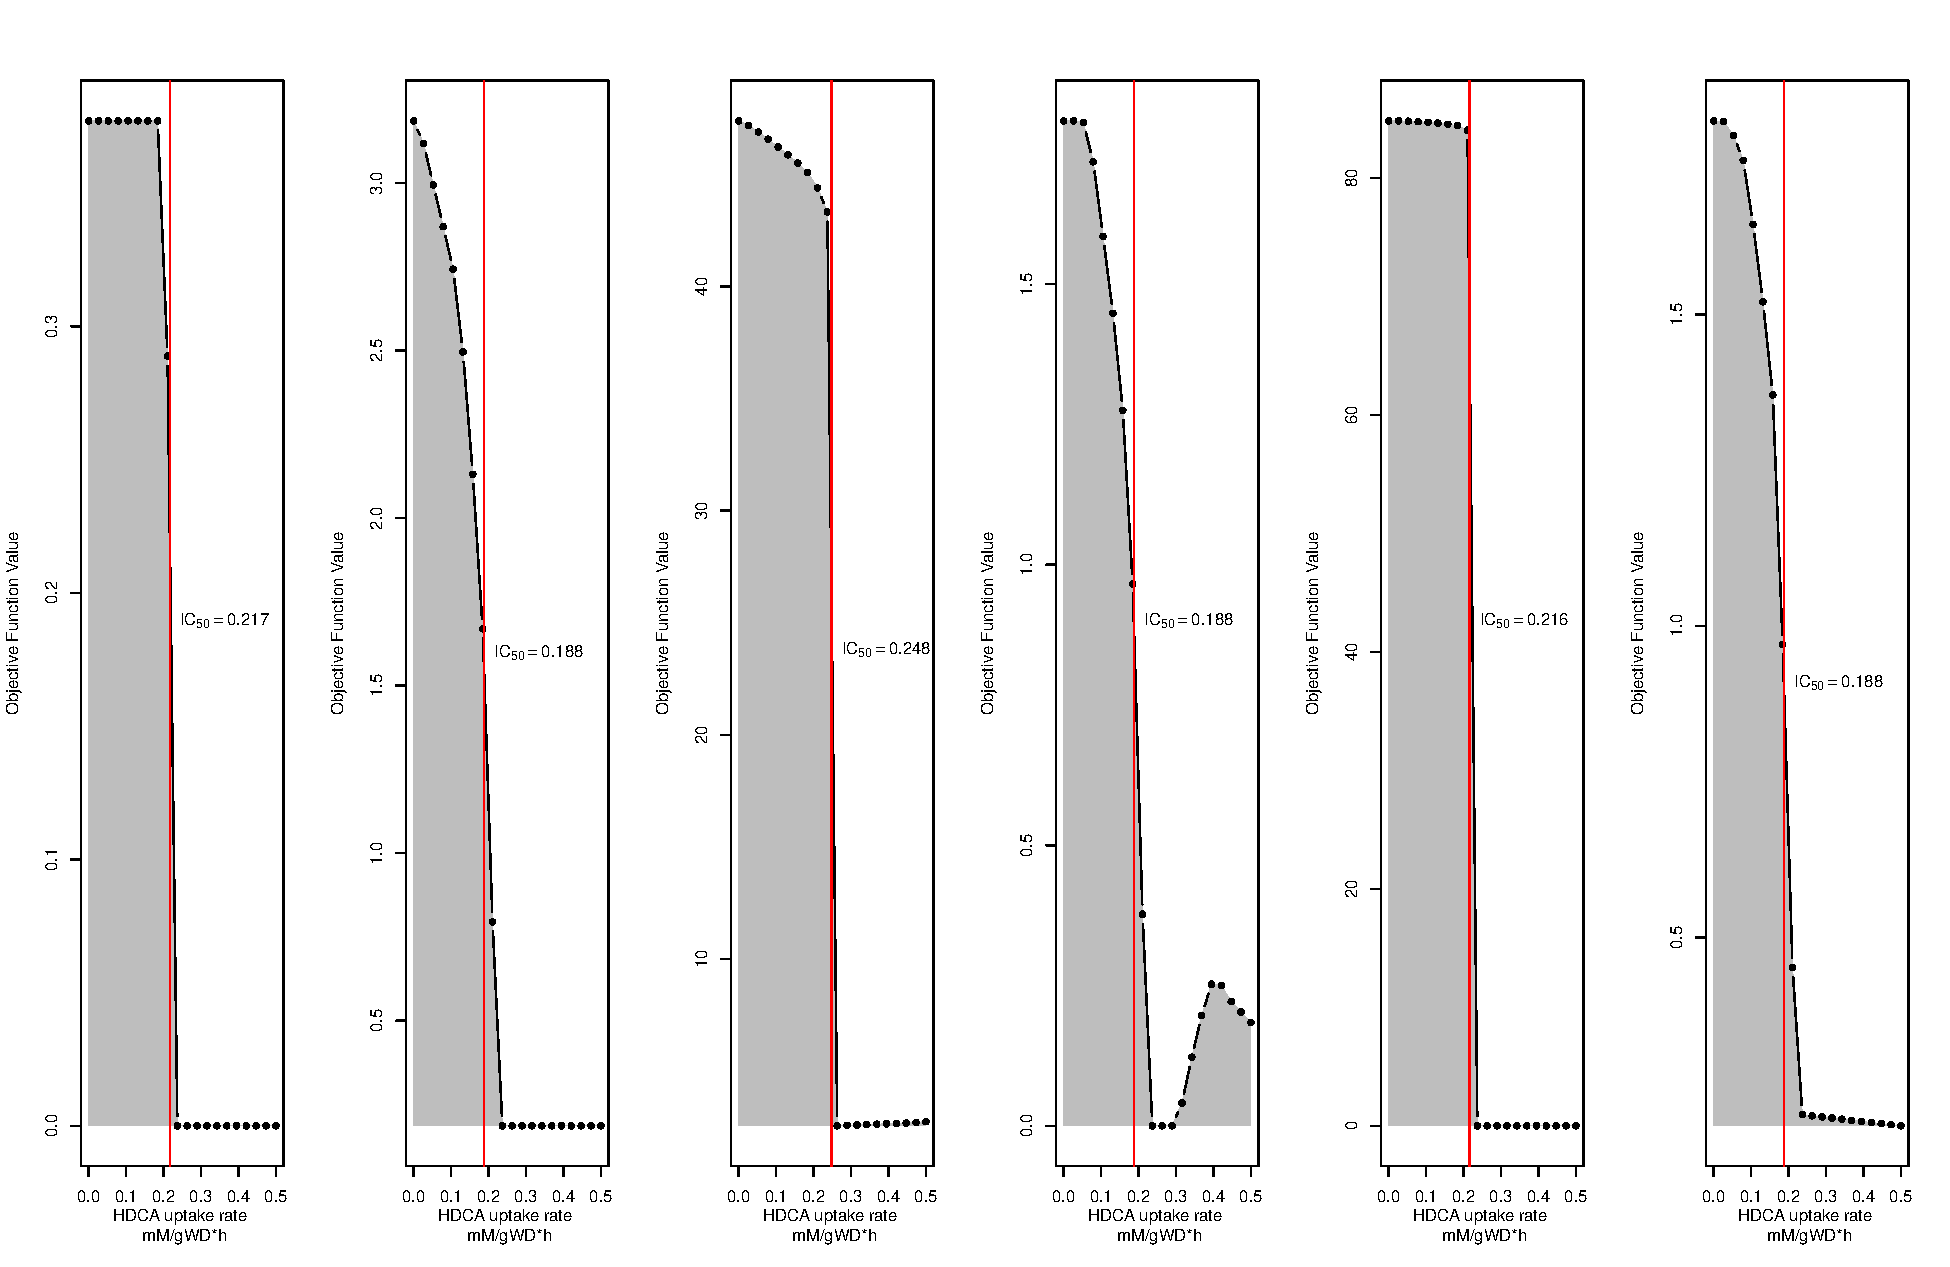
\includegraphics[width=0.95\textwidth]{IC50}\\
{\tiny Li Liu \textit{et al}. (2013) Palmitate-activated astrocytes via serine palmitoyltransferase increase BACE1 in primary neurons by sphingomyelinases.\\}
\end{center}
\end{frame}
\begin{frame}{Cellular Maintenance: Inflamed Scenario}
\begin{center}

\includegraphics[width=\textwidth]{I-results}\\
\end{center}
\textcolor{blue}{\textcircled{{\tiny 1}}} {\tiny Rachel Williams \textit{et al}. (2012). Pathogenic implications of iron accumulation in multiple sclerosis.\vspace{0.3cm}\\}\pause
\textcolor{blue}{\textcircled{{\tiny 2}}} {\tiny Mithilesh Kumar Jha \textit{et al}. (2016). Metabolic Control of Glia-Mediated Neuroinflammation.\vspace{0.1cm}\\}
\textcolor{blue}{\textcircled{{\tiny 2}}} {\tiny V Parpura and P G Haydon. (2000). Physiological astrocytic calcium levels stimulate glutamate release to modulate adjacent neurons.\vspace{0.1cm}\\}
\textcolor{blue}{\textcircled{{\tiny 2}}} {\tiny Leif Hertz \textit{et al}. (1999). Astrocytes: Glutamate producers for neurons.\vspace{0.1cm}\\}
\end{frame}
\begin{frame}{Cellular Maintenance: Inflamed Scenario}
\begin{center}

\includegraphics[width=\textwidth]{I-results}\\
\end{center}
\textcolor{blue}{\textcircled{{\tiny 3}}} {\tiny Yu-Cun Niu \textit{et al}. (2012). Histidine and arginine are associated with inflammation and oxidative stress in obese women. \vspace{0.1cm}\\}
\textcolor{blue}{\textcircled{{\tiny 4}}} {\tiny Leonard T. Rael \textit{et al}. (2004). An anti-inflammatory role for N-acetyl aspartate in stimulated human astroglial cells.\vspace{0.1cm}\\}
\textcolor{blue}{\textcircled{{\tiny 5}}} {\tiny D. R. Green \textit{et al}. (2014). Metabolic control of cell death.  \vspace{0.1cm}\\}
\end{frame}
\begin{frame}{Gliotransmitters}
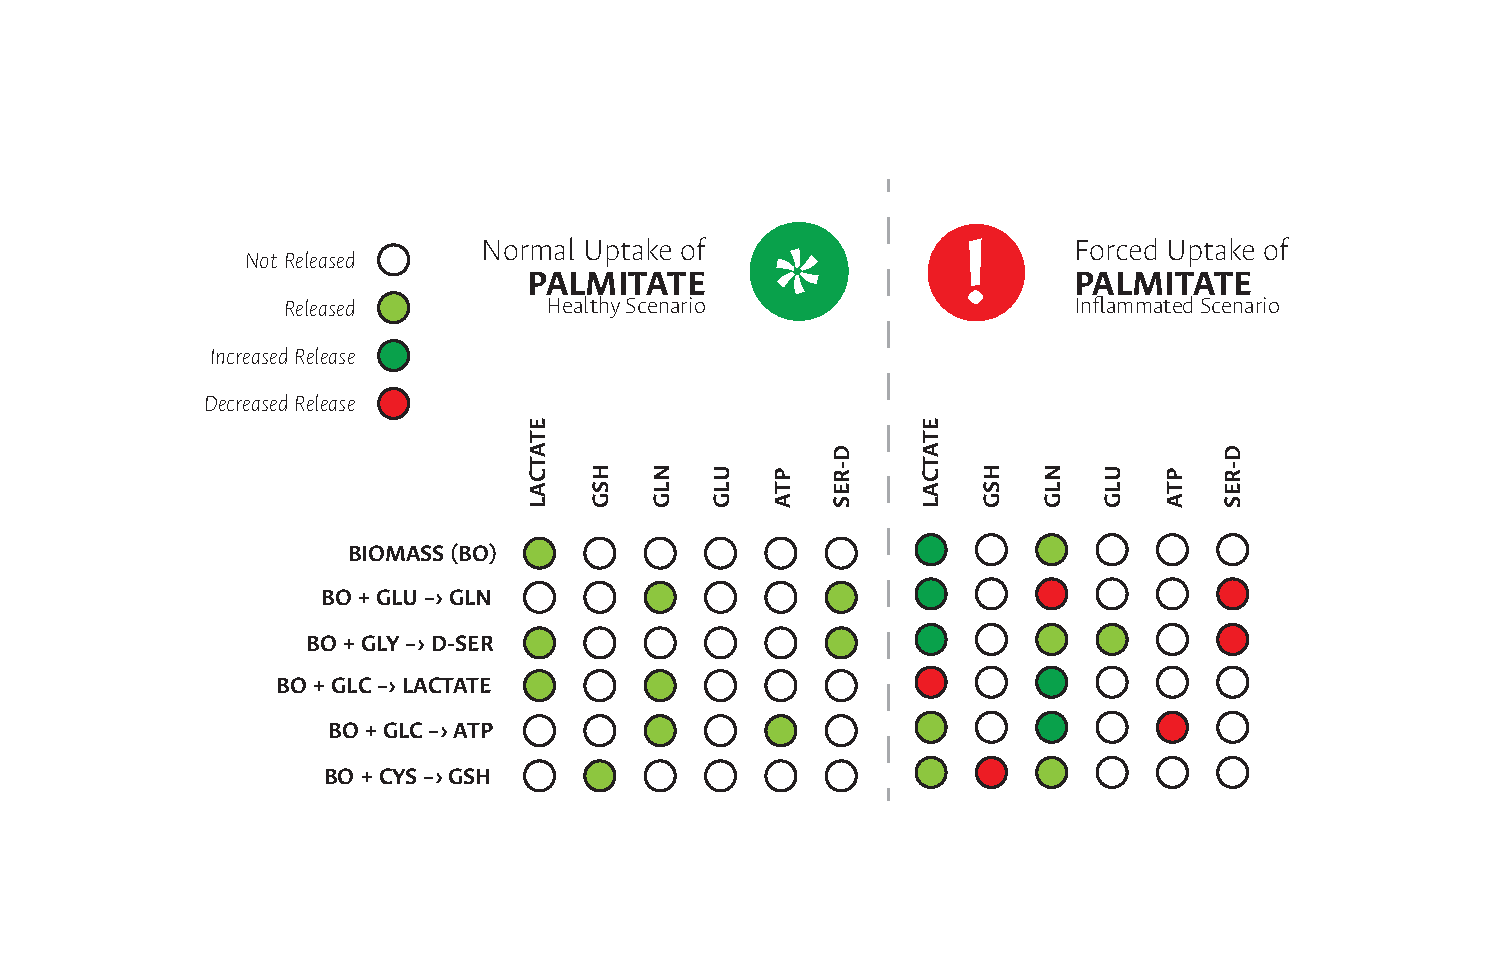
\includegraphics[width=\textwidth]{GTi}
\end{frame}
\begin{frame}{Anti-inflammatory Enzymes: : Innate defence against inflammation}
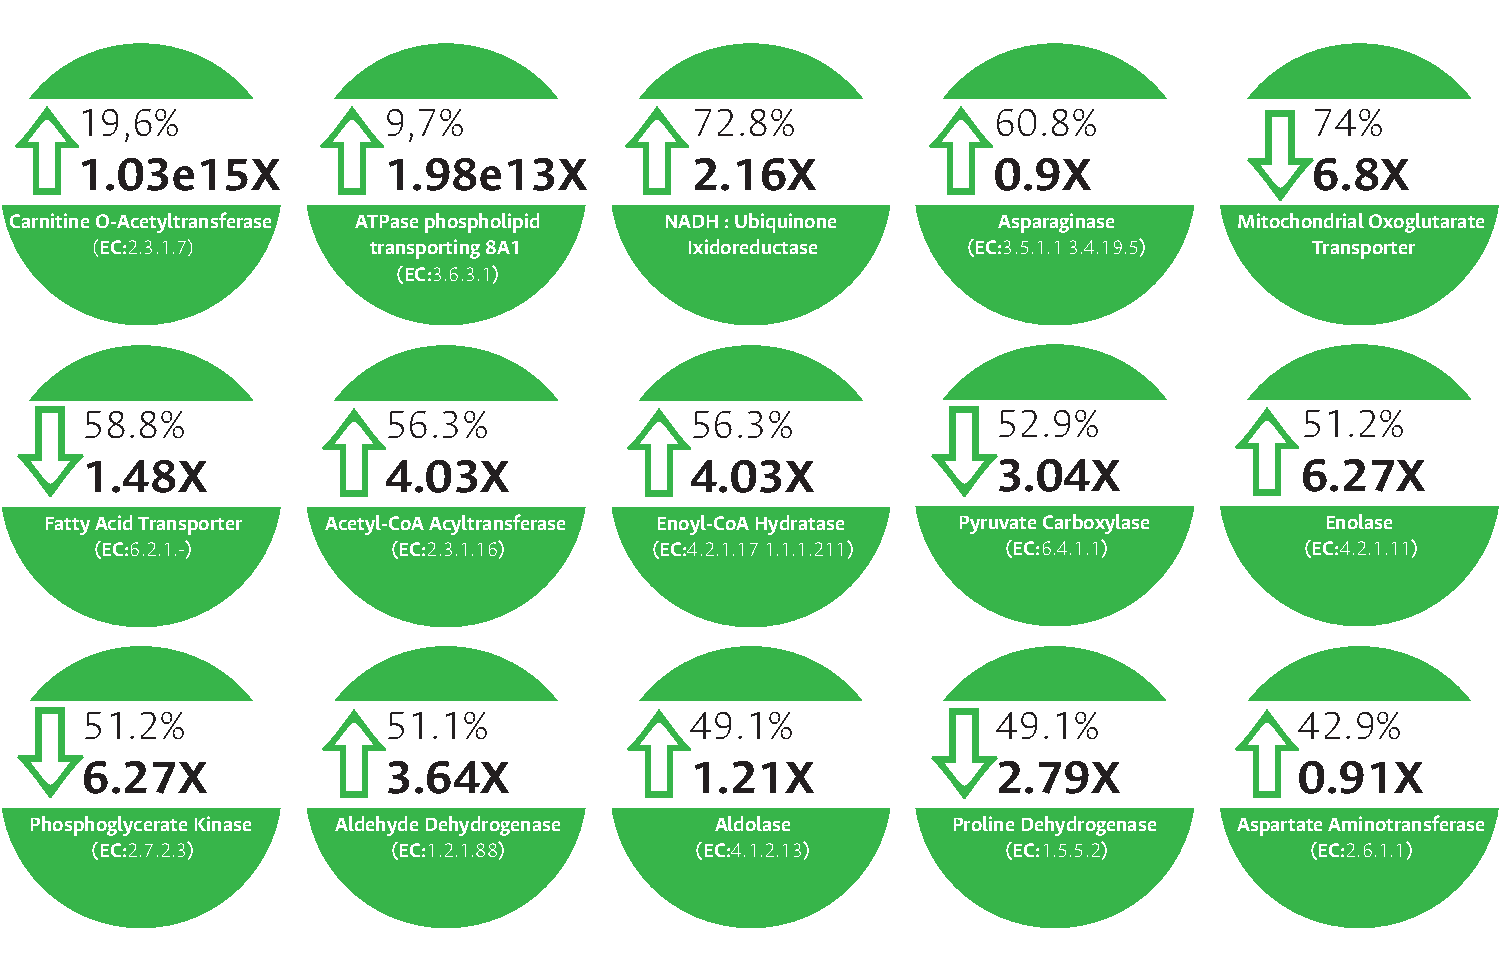
\includegraphics[width=\textwidth]{Antiinflammatory}
\end{frame}
\begin{frame}{Pro-inflammatory Enzymes}
\includegraphics[width=\textwidth]{Proinflammatory}
\end{frame}
\begin{frame}{Cellular Maintenance: Medicated Scenario}
\begin{center}
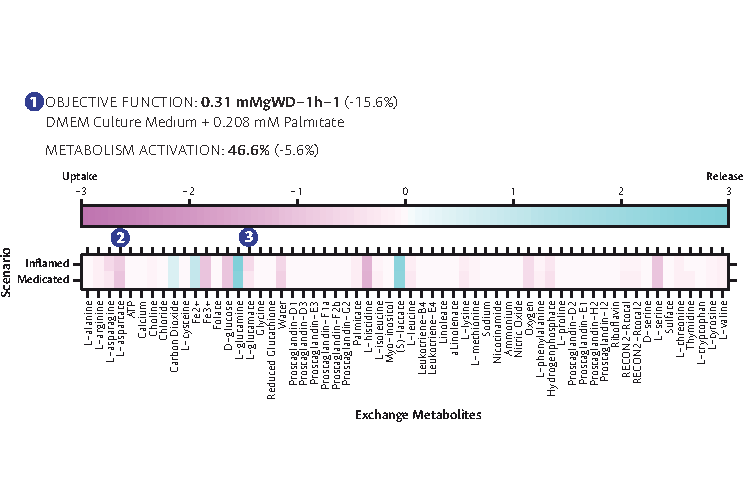
\includegraphics[width=\textwidth]{M-results}
\end{center}
\textcolor{blue}{\textcircled{{\tiny 1}}} {\tiny Kazuhiro Takuma, Akemichi Baba, and Toshio Matsuda. (2004). Astrocyte apoptosis: Implications for neuroprotection. \vspace{0.1cm}\\}
\textcolor{blue}{\textcircled{{\tiny 1}}} {\tiny Graham A., \textit{et al}. (1993). Hormone replacement therapy and risk of breast cancer: Results from epidemiologic studies. \vspace{0.1cm}\\}
\textcolor{blue}{\textcircled{{\tiny 1}}} {\tiny Graham A., \textit{et al}. (1995). The Use of Estrogens and Progestins and the Risk of Breast Cancer in Postmenopausal Women\\}
\end{frame}
\begin{frame}{Cellular Maintenance: Medicated Scenario}
\begin{center}
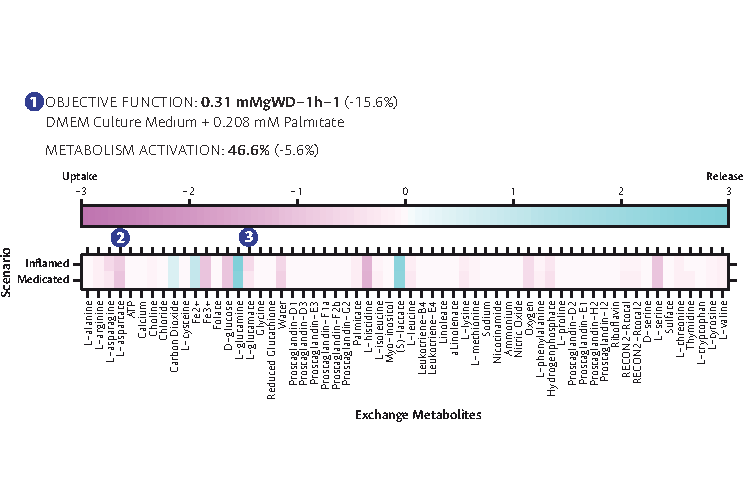
\includegraphics[width=\textwidth]{M-results}
\end{center}
\textcolor{blue}{\textcircled{{\tiny 2}}} {\tiny Leonard T. Rael \textit{et al}. (2004). An anti-inflammatory role for N-acetyl aspartate in stimulated human astroglial cells.\vspace{0.3cm}\\}\pause
\textcolor{blue}{\textcircled{{\tiny 3}}} {\tiny Francesco Petrelli and Paola Bezzi. (2016). Novel insights into gliotransmitters. \vspace{0.1cm}\\}
\textcolor{blue}{\textcircled{{\tiny 3}}} {\tiny Barbara Ahlemeyer \textit{et al}. (2002). Increase in glutamate-induced neurotoxicity by activated astrocytes involves stimulation of protein kinase C.\\}
\end{frame}
\begin{frame}{Gliotransmitters}
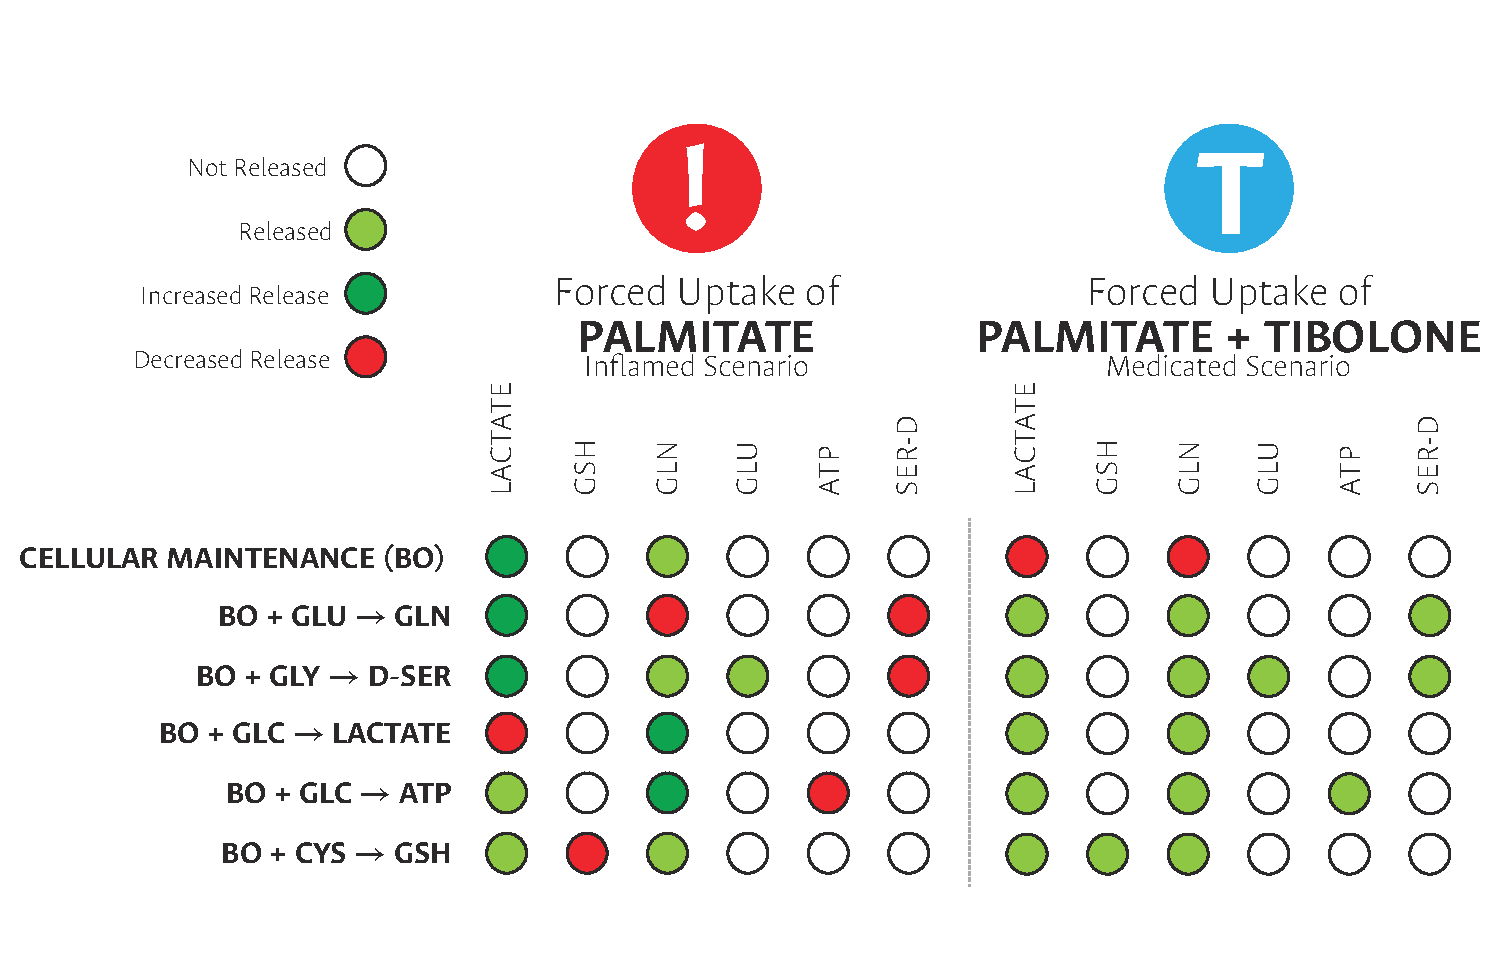
\includegraphics[width=\textwidth]{GTt}
\end{frame}
\begin{frame}{Tibolone Related Enzymes}
\begin{center}
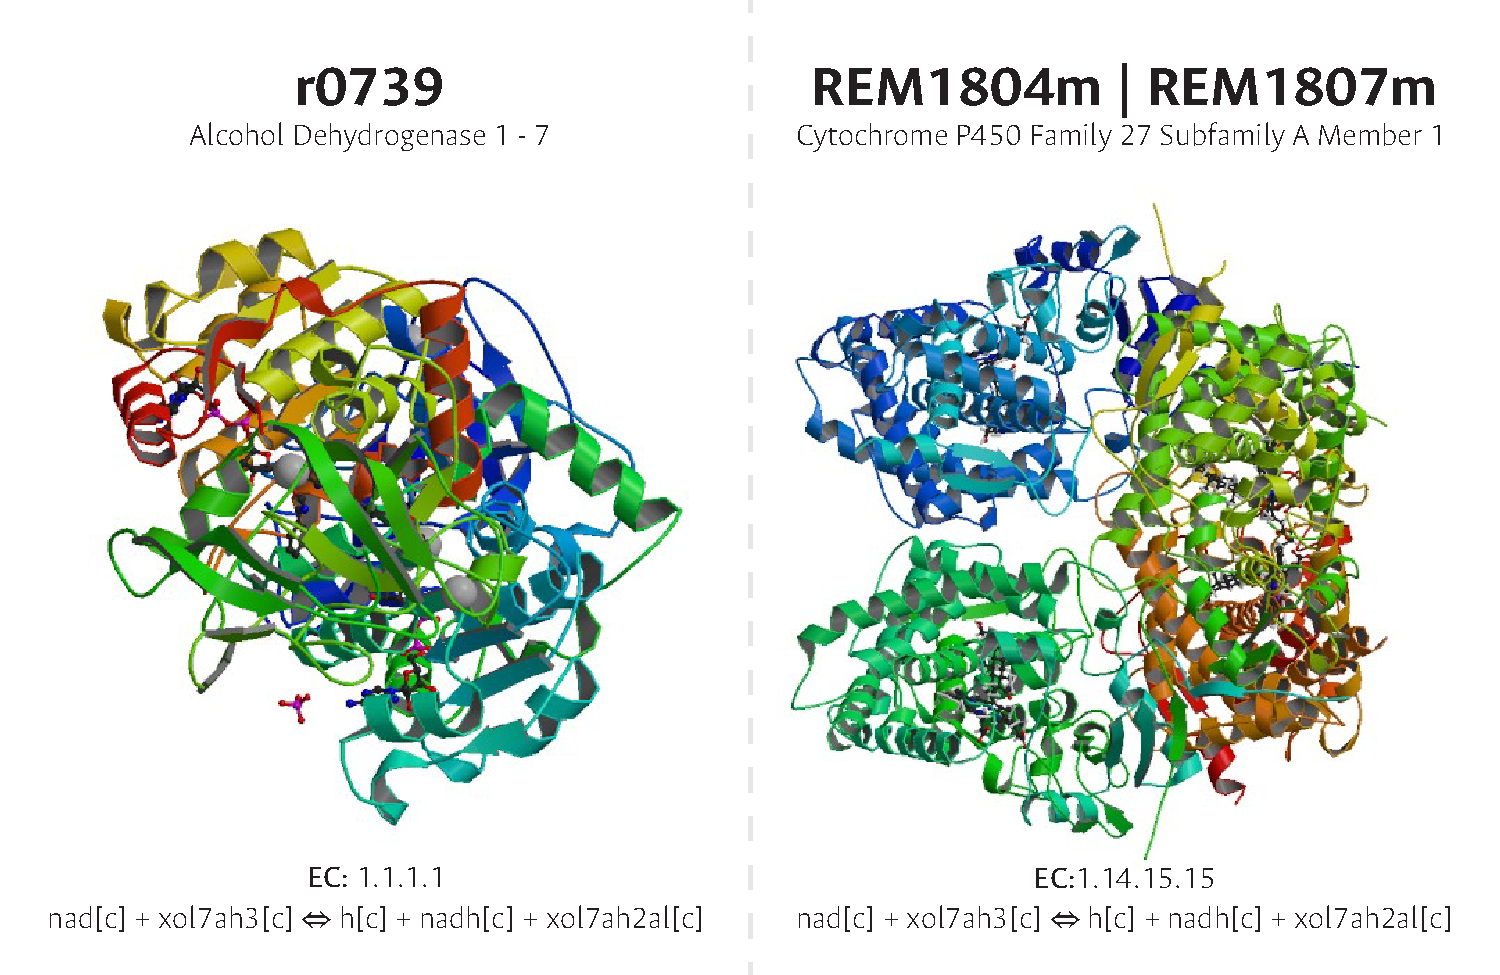
\includegraphics[width=\textwidth]{TiboloneEnzymes}
\end{center}
{\scriptsize F. Sun \textit{et al}. (2009). Inhibitory effect of osthole on alcohol-induced fatty liver in mice.}
\end{frame}
\begin{frame}{Reproducibility}
\begin{center}
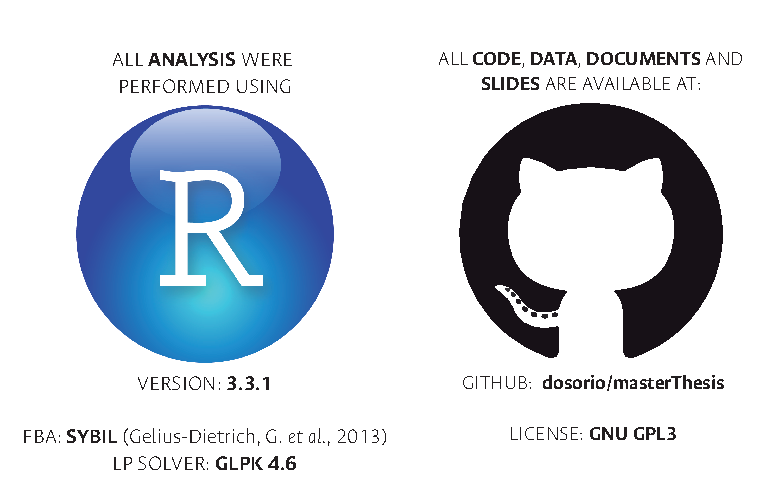
\includegraphics[width=\textwidth]{Materials}
\end{center}
\end{frame}
\section{Conclusions}
\begin{frame}{Conclusions}
\begin{center}
\begin{enumerate}
\item  A tissue-specific metabolic reconstruction for mature astrocytes has been developed and on it, three different metabolic scenarios were modeled.
\item The metabolic model was capable of yielding results which were in correspondence to the experimentally proved metabolic processes.
\item Adverse effects associated with the increase of palmitate uptake were described based on exchange, metabolite production, and metabolic pathways perturbed under the inflammatory response.
\item Two possible reactions and their associated enzymes susceptible to be knocked out to reduce the metabolic inflammation were identified.
\end{enumerate}
\end{center}
\end{frame}
\begin{frame}{Conclusions}
\begin{center}
\begin{enumerate}
\item[5.]  Based on literature reports a tibolone medicated scenario was modeled and used to identify and describe the neuroprotective effects of this synthetic neurosteroid under an inflamed scenario in mature astrocytes.
\item[6.] Our main results suggest that tibolone execute their neuroprotective effects through a reduction of neurotoxicity mediated by L-glutamate in mature astrocytes.
\item[7.] We found a tibolone associated increase in growth rate probably in concordance to previously reported side effects of steroids in other human cell types.
\end{enumerate}
\end{center}
\end{frame}
\section{Publications}
\begin{frame}{Published Software Packages}
\begin{center}
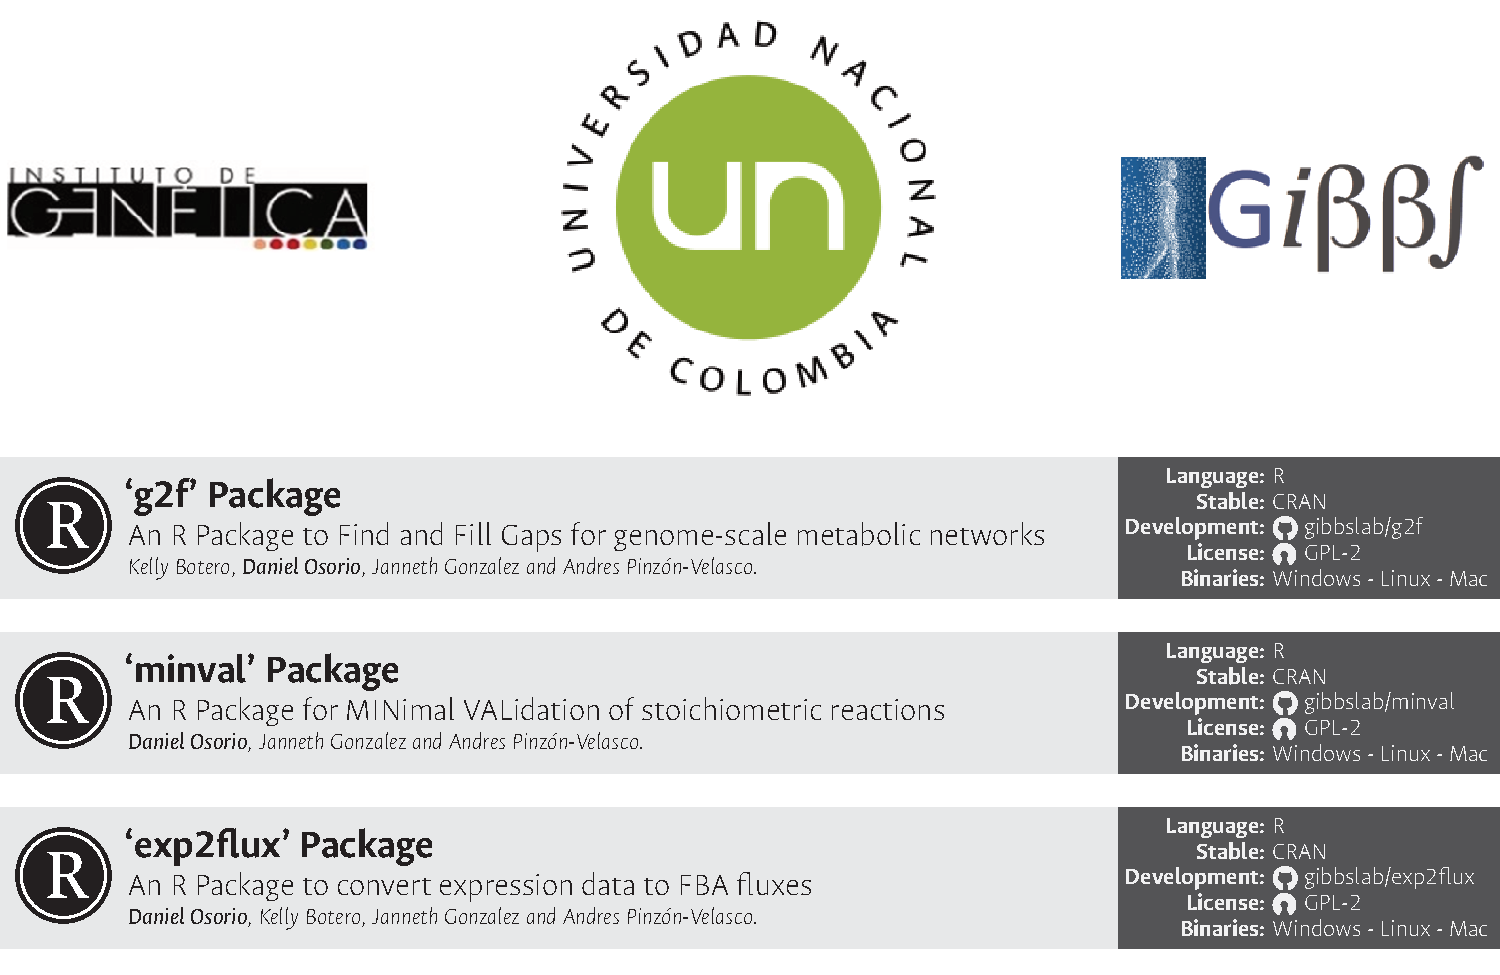
\includegraphics[width=\textwidth]{SPackages}
\end{center}
\end{frame}
\begin{frame}{This work is a set of four manuscripts}
\begin{footnotesize}
\begin{description}
\item[ACCEPTED WITH CORRECTIONS] Osorio, D., Gonzalez, J., and Pinzón-Velasco, A. \textbf{minval: An R package for MINimal VALidation of stoichiometric reactions.} \textit{The R Journal}.
\item[IN PREPARATION] Osorio, D., Botero, K., Gonzalez, J., and Pinzón-Velasco, A. \textbf{exp2flux: An R package to convert expression data to FBA fluxes.} To be submitted to \textit{The R Journal}
\item[IN PREPARATION] Osorio, D., Gonzalez, J., and Pinzón-Velasco, A.\textbf{ Exploring the neuroprotective effects of tibolone during astrocytic metabolic inflammation: a flux balance analysis approach.} To be submitted to \textit{Medical Hypotheses}
\item[IN PREPARATION] Botero, K., Osorio, D., Gonzalez, J., and Pinzón-Velasco, A. \textbf{g2f: An R packafe to find and fill gaps for genome-scale metabolic networks.} To be submitted to \textit{The R Journal}
\end{description}
\end{footnotesize}
\end{frame}
\section{Events}
\begin{frame}{Advances of this work were presented as:}
\begin{center}
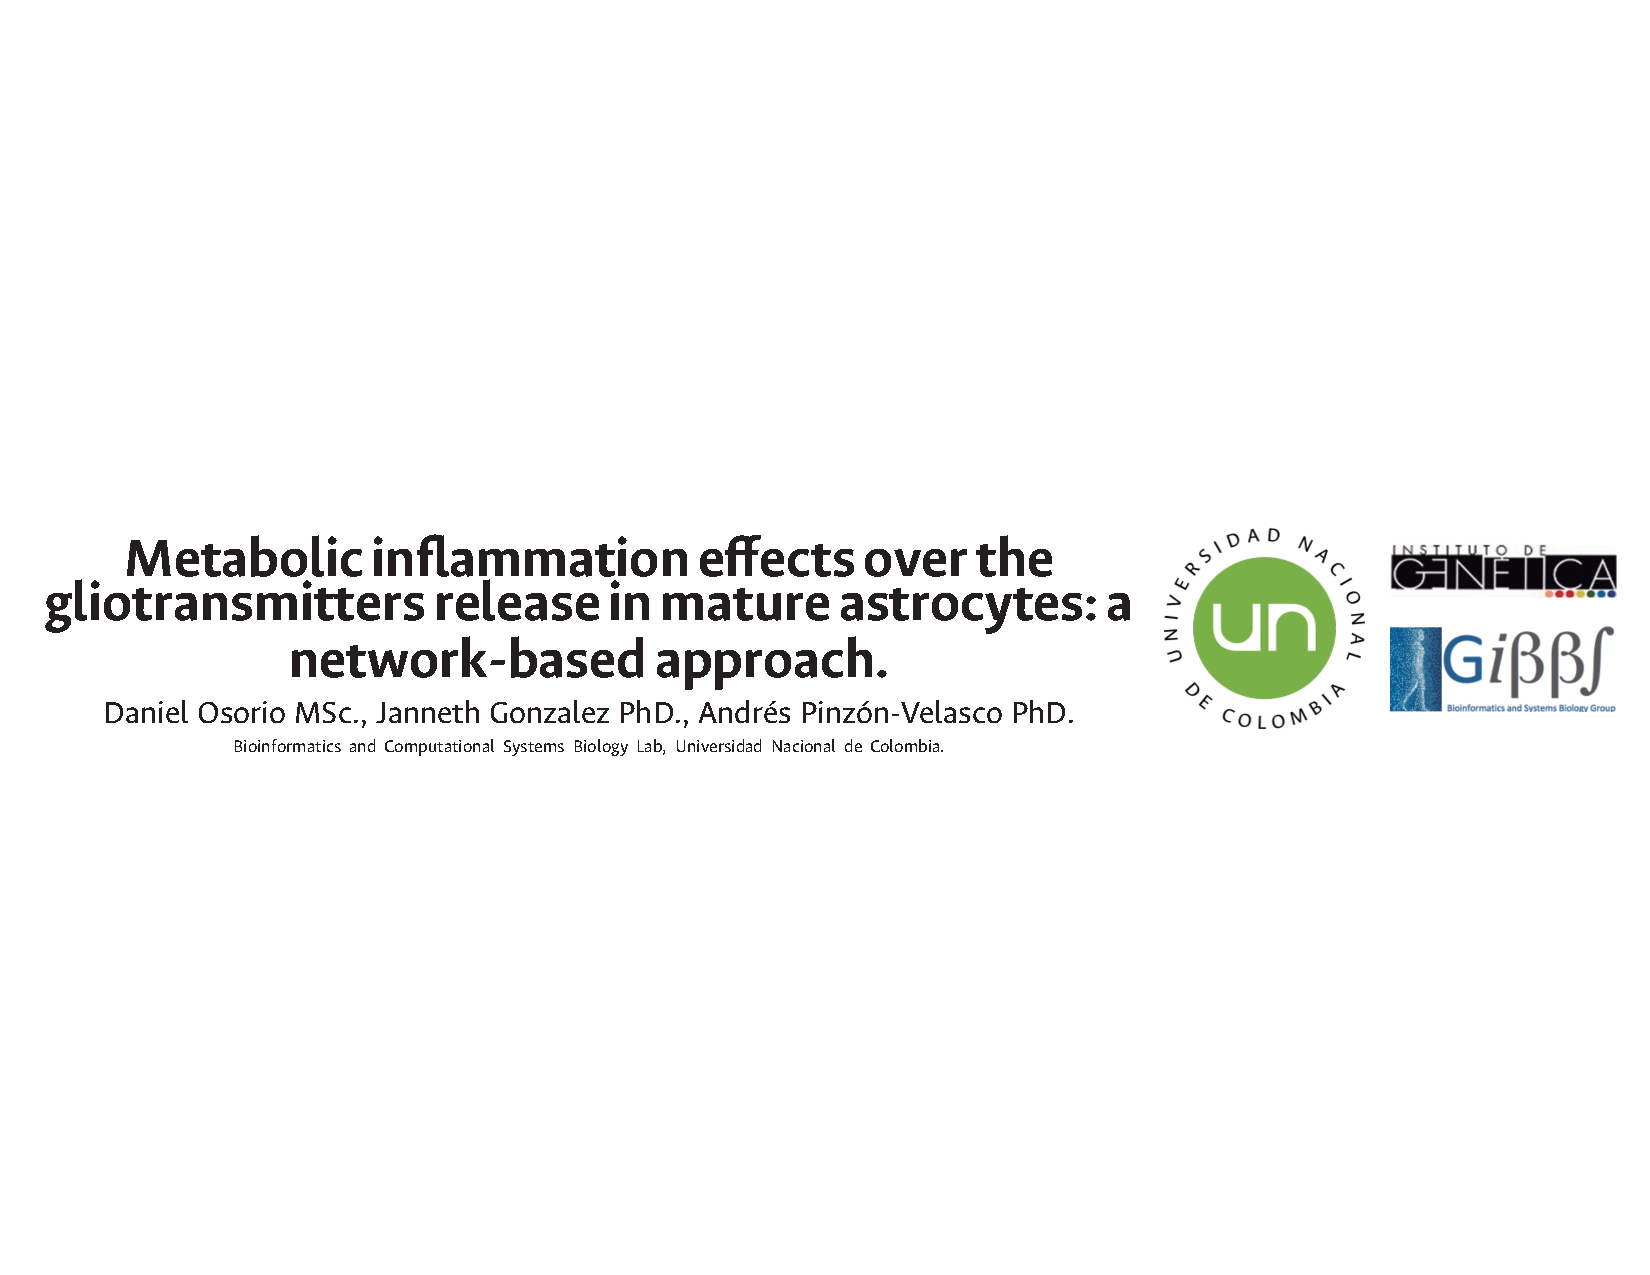
\includegraphics[width=\textwidth]{Events}
\end{center}
\hrulefill \ at: \hrulefill
\begin{multicols}{3}
\begin{center}
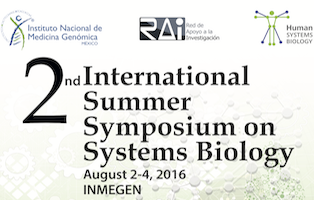
\includegraphics[width=0.3\textwidth]{IS3B}\\
CDMX, México\\
\textbf{Short Talk}
\end{center}
\begin{center}
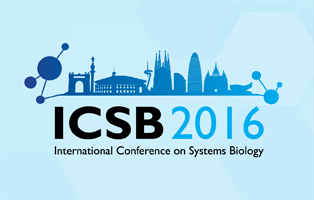
\includegraphics[width=0.3\textwidth]{ICSB}\\
Barcelona, España\\
\textbf{Poster}
\end{center}
\begin{center}

\includegraphics[width=0.3\textwidth]{ICGEB}\\
Bogotá, Colombia\\
\textbf{Short Talk}
\end{center}
\end{multicols}
\end{frame}
\section{Acknowledgements}
\begin{frame}{Acknowledgements}
\begin{center}

\includegraphics[height=1.8cm]{UN}\hspace{0.5cm}

\includegraphics[height=1.8cm]{Javeriana}\vspace{0.5cm}\\
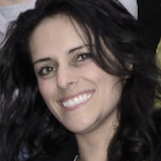
\includegraphics[width=2.7cm]{Janneth}
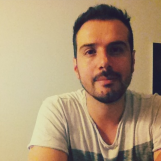
\includegraphics[width=2.7cm]{Andres}
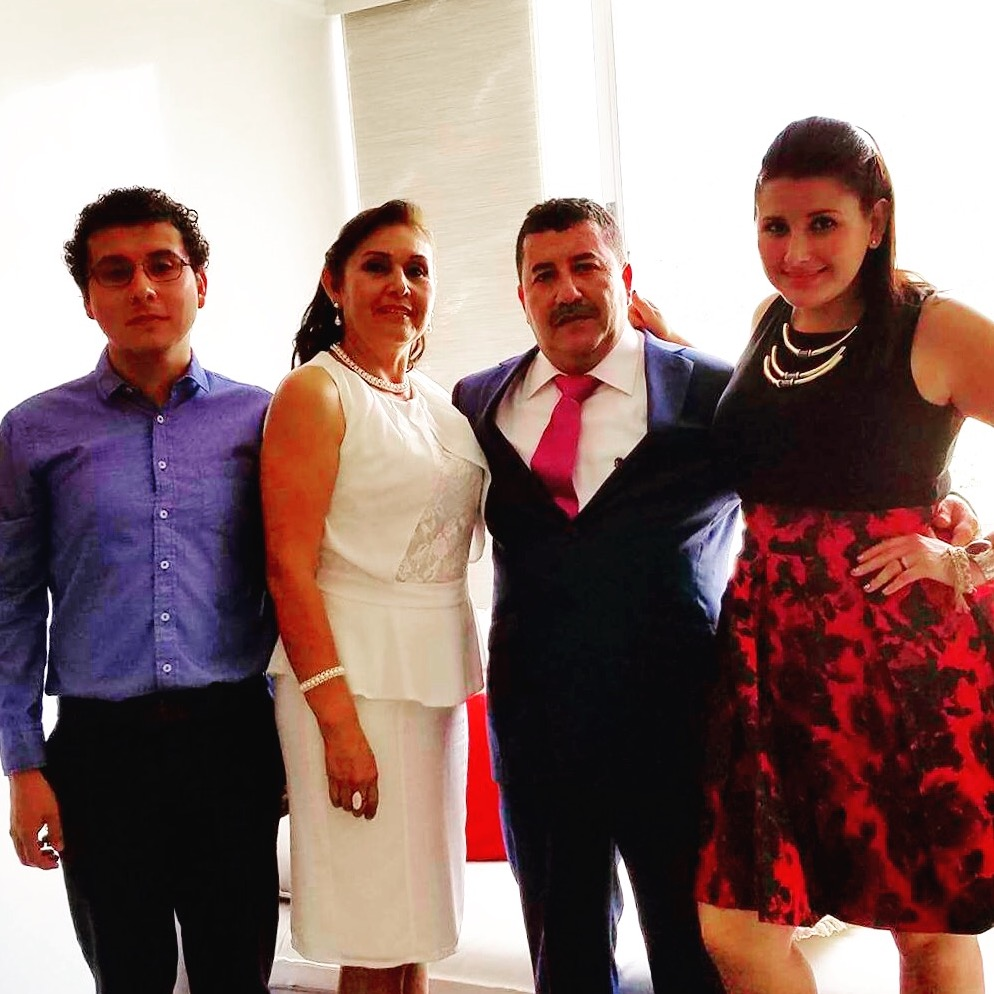
\includegraphics[width=2.7cm]{Familia}
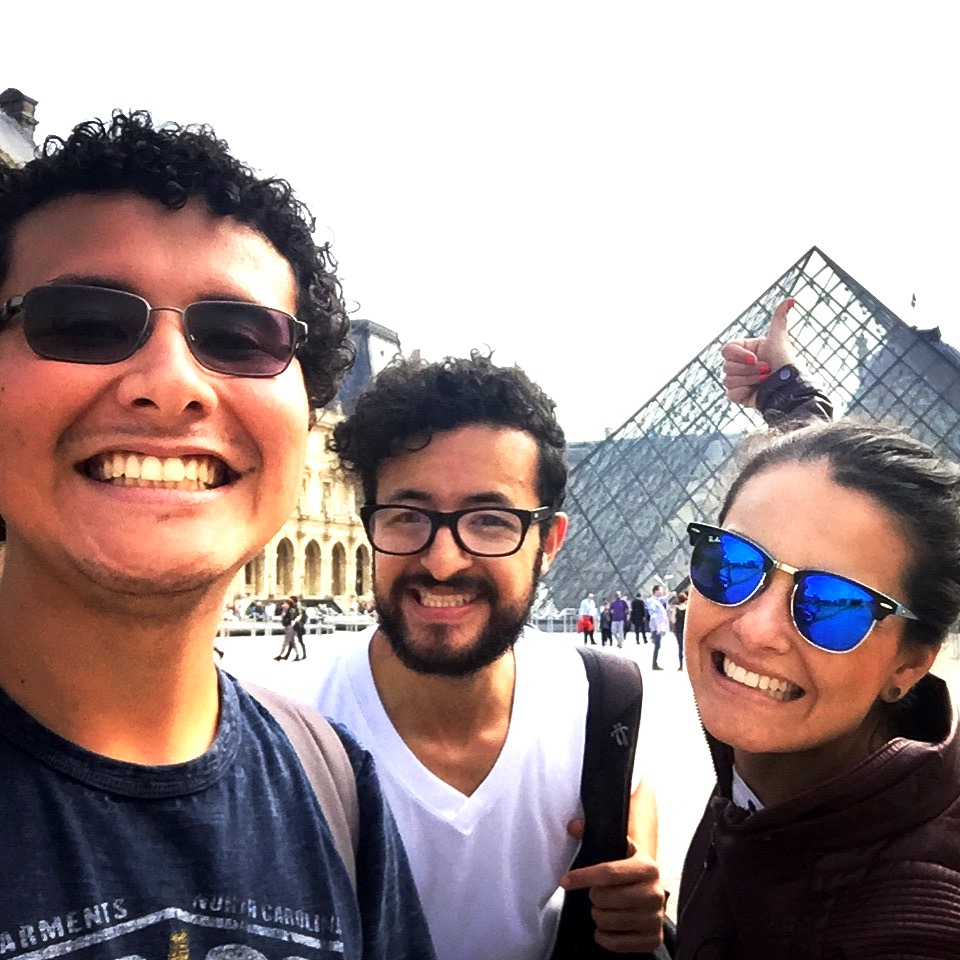
\includegraphics[width=2.7cm]{Kelly-Juan-Daniel}\\
\end{center}
\end{frame}
\section{Questions}
\begin{frame}{Thanks to be here!}
\begin{multicols}{2}

\includegraphics[height=0.7cm]{logoIG}
\begin{flushright}
\includegraphics[height=0.7cm]{logoGIBBS}
\end{flushright}
\end{multicols}
\begin{center}
This study was developed at the:\\
\includegraphics[width=\textwidth]{GIBBS}\\
\textbf{Bioinformatics and Computational Systems Biology Lab}\\
Institute for Genetics - Universidad Nacional de Colombia
\end{center}
\begin{multicols}{2}
\begin{center}
\textbf{Daniel Osorio}\\
dcosorioh@unal.edu.co\\
\textbf{Andrés Pinzón PhD}\\
ampinzonv@unal.edu.co
\end{center}
\end{multicols}
\end{frame}
\end{document}
